% ============================================================
% CHƯƠNG 4: THỰC NGHIỆM VÀ KẾT QUẢ
% ============================================================
\chapter{Thực nghiệm và kết quả}
\label{chap:experiments}

\section{Cấu hình thực nghiệm}
\label{sec:experiment_setup}

Toàn bộ thực nghiệm được thực hiện trên cùng một cấu hình phần cứng và phần mềm:

\begin{table}[H]
\centering
\caption{Cấu hình môi trường thực nghiệm}
\label{tab:env_config}
\begin{tabular}{ll}
\toprule
\textbf{Thành phần} & \textbf{Chi tiết} \\
\midrule
GPU & NVIDIA GeForce RTX 3060 (12GB VRAM) \\
Python & 3.10 (Miniforge / Conda) \\
Framework & PyTorch 1.6+ \\
Optimizer & AdamW \\
Learning rate & $10^{-4}$ \\
Batch size & 64 \\
Số epochs & 60 \\
Random seed & 100 \\
Phân chia dữ liệu & Speaker-Independent (val=1F, test=1M) \\
\bottomrule
\end{tabular}
\end{table}

Hệ thống tự động lưu các artifact sau mỗi lượt huấn luyện bao gồm trọng số mô hình tốt nhất dạng tệp tin \texttt{.pth}, biểu đồ thể hiện các đường cong học tập (learning curves) lưu dưới dạng ảnh \texttt{*\_curves.png}, và ma trận nhầm lẫn (confusion matrix) dạng heatmap lưu dưới dạng ảnh \texttt{*\_conf.png}.


\section{Kết quả thực nghiệm chính}
\label{sec:main_results}

\subsection{Bảng tổng hợp kết quả}

Bảng~\ref{tab:main_results} trình bày kết quả đánh giá trên tập test (Speaker 1M) cho tất cả 6 cấu hình mô hình. 

\begin{table}[H]
\centering
\setlength{\tabcolsep}{4.5pt}
\caption{Kết quả thực nghiệm trên tập test (val=1F, test=1M)}
\label{tab:main_results}
\begin{tabular}{clllrrrr}
\toprule
\textbf{\#} & \textbf{Mô hình} & \textbf{Loss} & \textbf{Aug.} & \textbf{Params} & \textbf{Test Loss} & \textbf{WA (\%)} & \textbf{UA (\%)} \\
\midrule
1 & AlexNet (Baseline) & CE & Không & 57,02M & 1,2138 & 50,73 & 25,00 \\
2 & AlexNet GAP & CE & Không & 2,47M & 0,9859 & 78,54 & 64,89 \\
3 & ResNet-18 & Focal & EMix-S & 11,18M & 0,4541 & 76,10 & 64,37 \\
4 & DenseNet-121 & Focal & EMix-S & 6,96M & 0,2927 & 68,78 & 66,48 \\
5 & \textbf{EfficientNet-B0} $\star$ & \textbf{Focal} & \textbf{EMix-S} & \textbf{4,01M} & \textbf{0,2792} & \textbf{80,98} & \textbf{74,25} \\
6 & MobileNet-V2 & Focal & EMix-S & 2,23M & 0,3549 & 76,59 & 71,15 \\
\bottomrule
\end{tabular}
\end{table}

Trong số các mô hình đánh giá, cấu hình phối hợp EfficientNet-B0 cùng hàm lỗi Focal Loss và kỹ thuật tăng cường dữ liệu EMix-S mang lại hiệu năng tối ưu nhất trên lượt kiểm thử đơn lẻ này, đạt WA=80,98\% và UA=74,25\%. Tuy nhiên, cần nhận thức rằng thiết lập đánh giá trên một lượt chia (Single Fold) này chịu ảnh hưởng lớn bởi độ dễ/khó ngẫu nhiên của đặc trưng người nói kiểm thử (Speaker 1M) và chưa mang ý nghĩa thống kê đầy đủ do mẫu kiểm thử cảm xúc (như Anger và Happiness) rất hạn chế.

Một điểm đáng chú ý khác trong bảng kết quả baseline là khi so sánh hai mô hình dùng Cross Entropy thuần túy và không có tăng cường dữ liệu: phiên bản AlexNet GAP cải tiến (đạt 64,89\% UA) hoạt động tốt hơn đáng kể so với EfficientNet-B0 cơ sở (chỉ đạt 58,46\% UA, xem Mục~\ref{sec:ablation}). Điều này cho thấy với một bài toán có lượng dữ liệu nhỏ như SER, các mô hình học sâu hiện đại và phức tạp như EfficientNet-B0 rất dễ rơi vào trạng thái quá khớp (overfitting) nếu không có các kỹ thuật điều hòa hoặc tăng cường dữ liệu đi kèm, trong khi cấu hình tích hợp GAP của AlexNet hoạt động ổn định và bền bỉ hơn.

\subsection{Biểu đồ so sánh tổng hợp}

Các biểu đồ trực quan hóa kết quả so sánh giữa các mô hình được thể hiện từ Hình~\ref{fig:comparison_wa_ua} đến Hình~\ref{fig:summary}. Trong đó, Hình~\ref{fig:comparison_wa_ua} biểu diễn độ chính xác WA và UA của cả 6 cấu hình mô hình; Hình~\ref{fig:comparison_params} thể hiện mối quan hệ và sự cân bằng giữa số lượng tham số huấn luyện (model parameters) và Weighted Accuracy; và Hình~\ref{fig:summary} cung cấp cái nhìn tổng hợp về cả độ chính xác tổng thể và độ chính xác chi tiết theo từng lớp cảm xúc.

\begin{figure}[H]
    \centering
    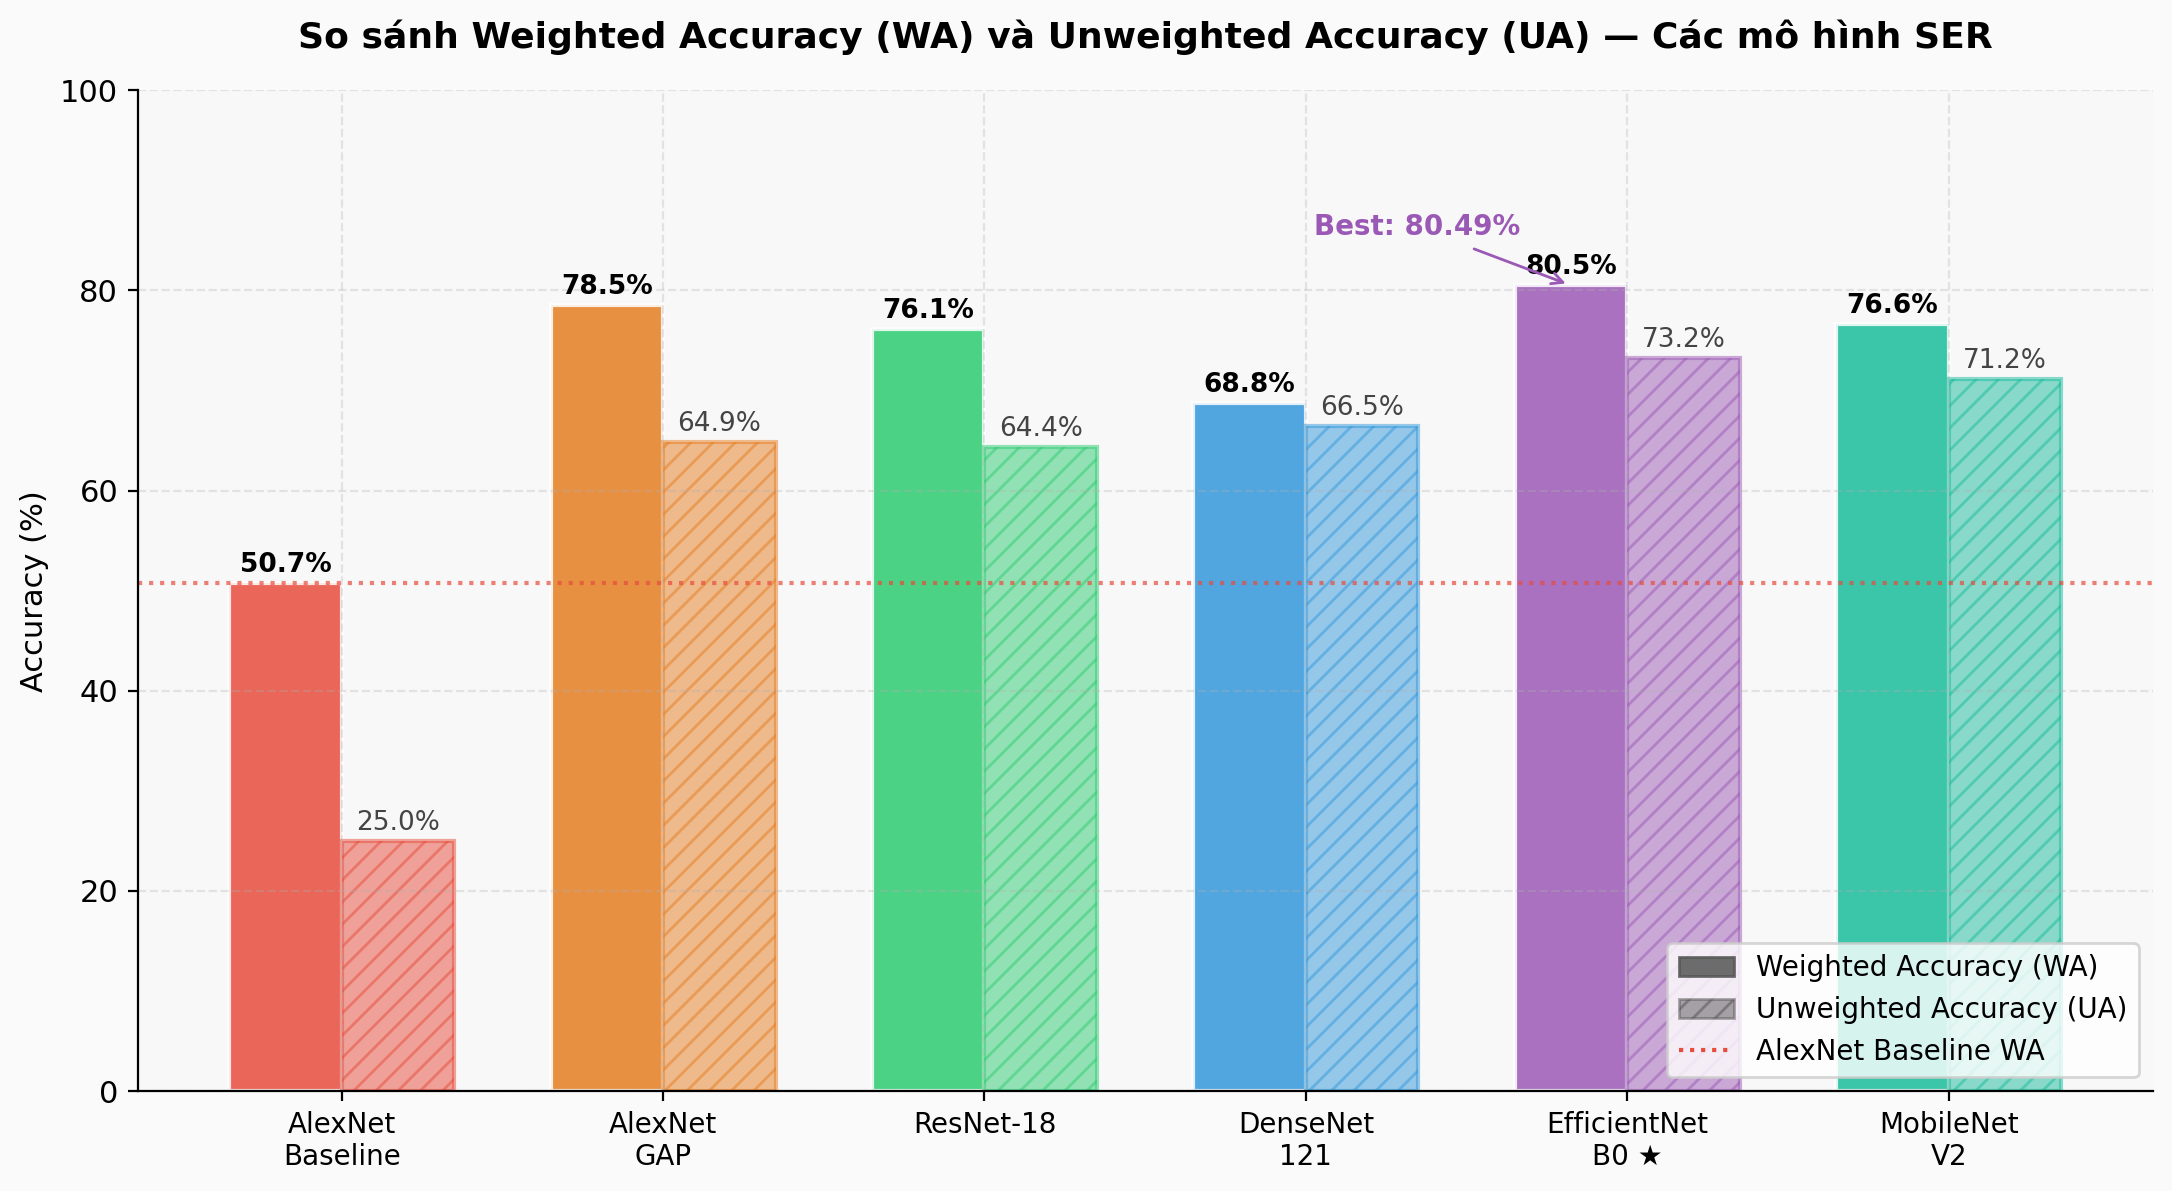
\includegraphics[width=0.85\textwidth]{comparison_wa_ua.png}
    \caption{Biểu đồ so sánh WA và UA giữa các mô hình}
    \label{fig:comparison_wa_ua}
\end{figure}

\begin{figure}[H]
    \centering
    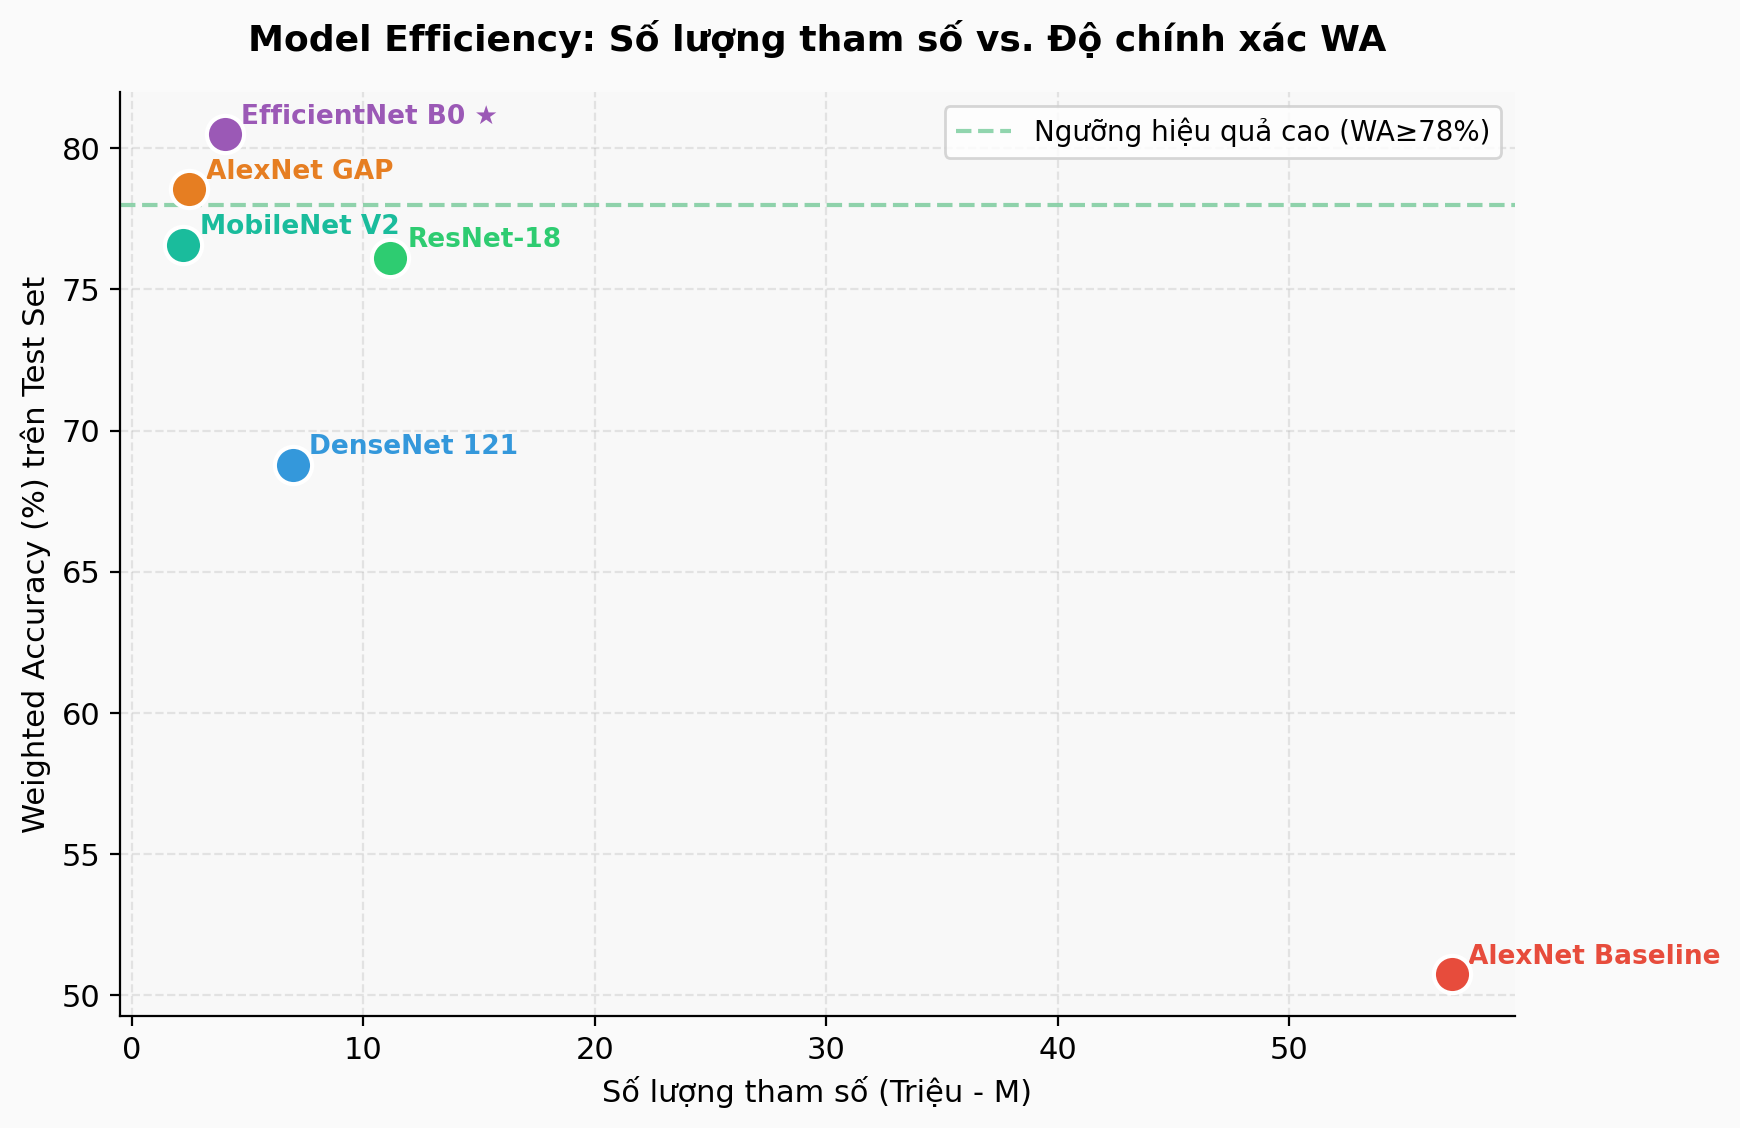
\includegraphics[width=0.85\textwidth]{comparison_params_vs_wa.png}
    \caption{Mối quan hệ giữa số lượng tham số và Weighted Accuracy}
    \label{fig:comparison_params}
\end{figure}

\begin{figure}[H]
    \centering
    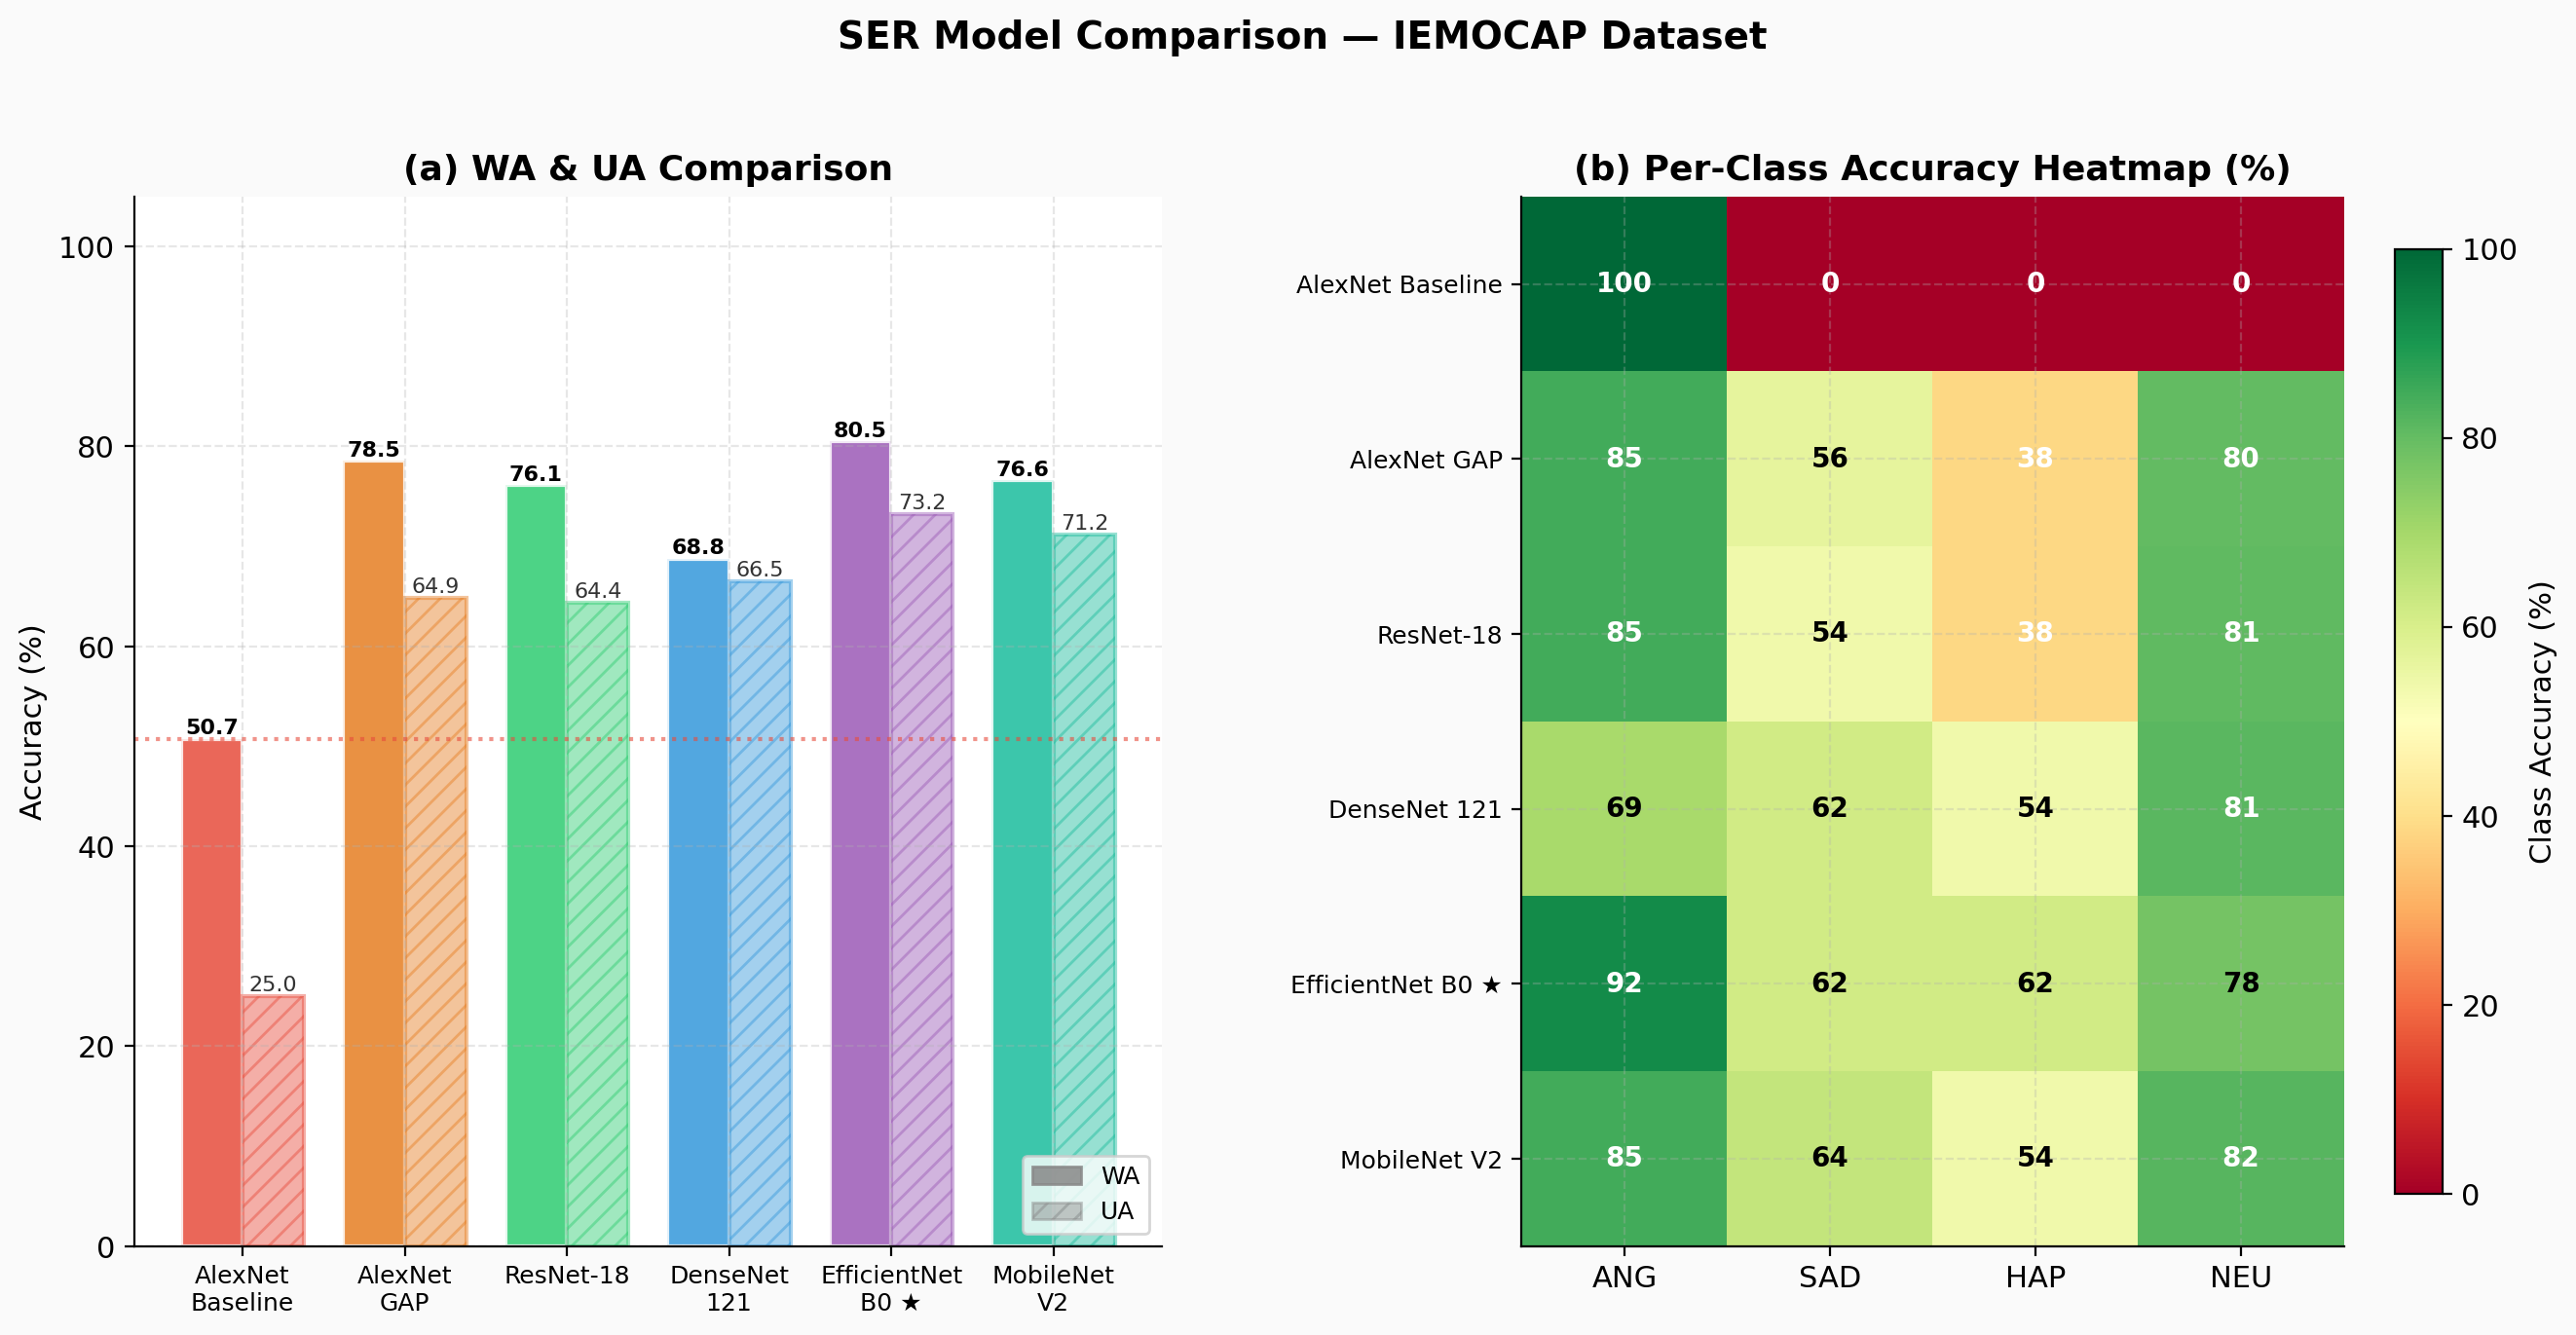
\includegraphics[width=\textwidth]{summary_figure.png}
    \caption{Biểu đồ tổng hợp kết quả thực nghiệm (publication-quality)}
    \label{fig:summary}
\end{figure}


\section{Phân tích chi tiết từng mô hình}
\label{sec:detailed_analysis}

\subsection{AlexNet Baseline (Cross Entropy, Không Augmentation)}

\begin{figure}[H]
    \centering
    \begin{subfigure}[b]{0.55\textwidth}
        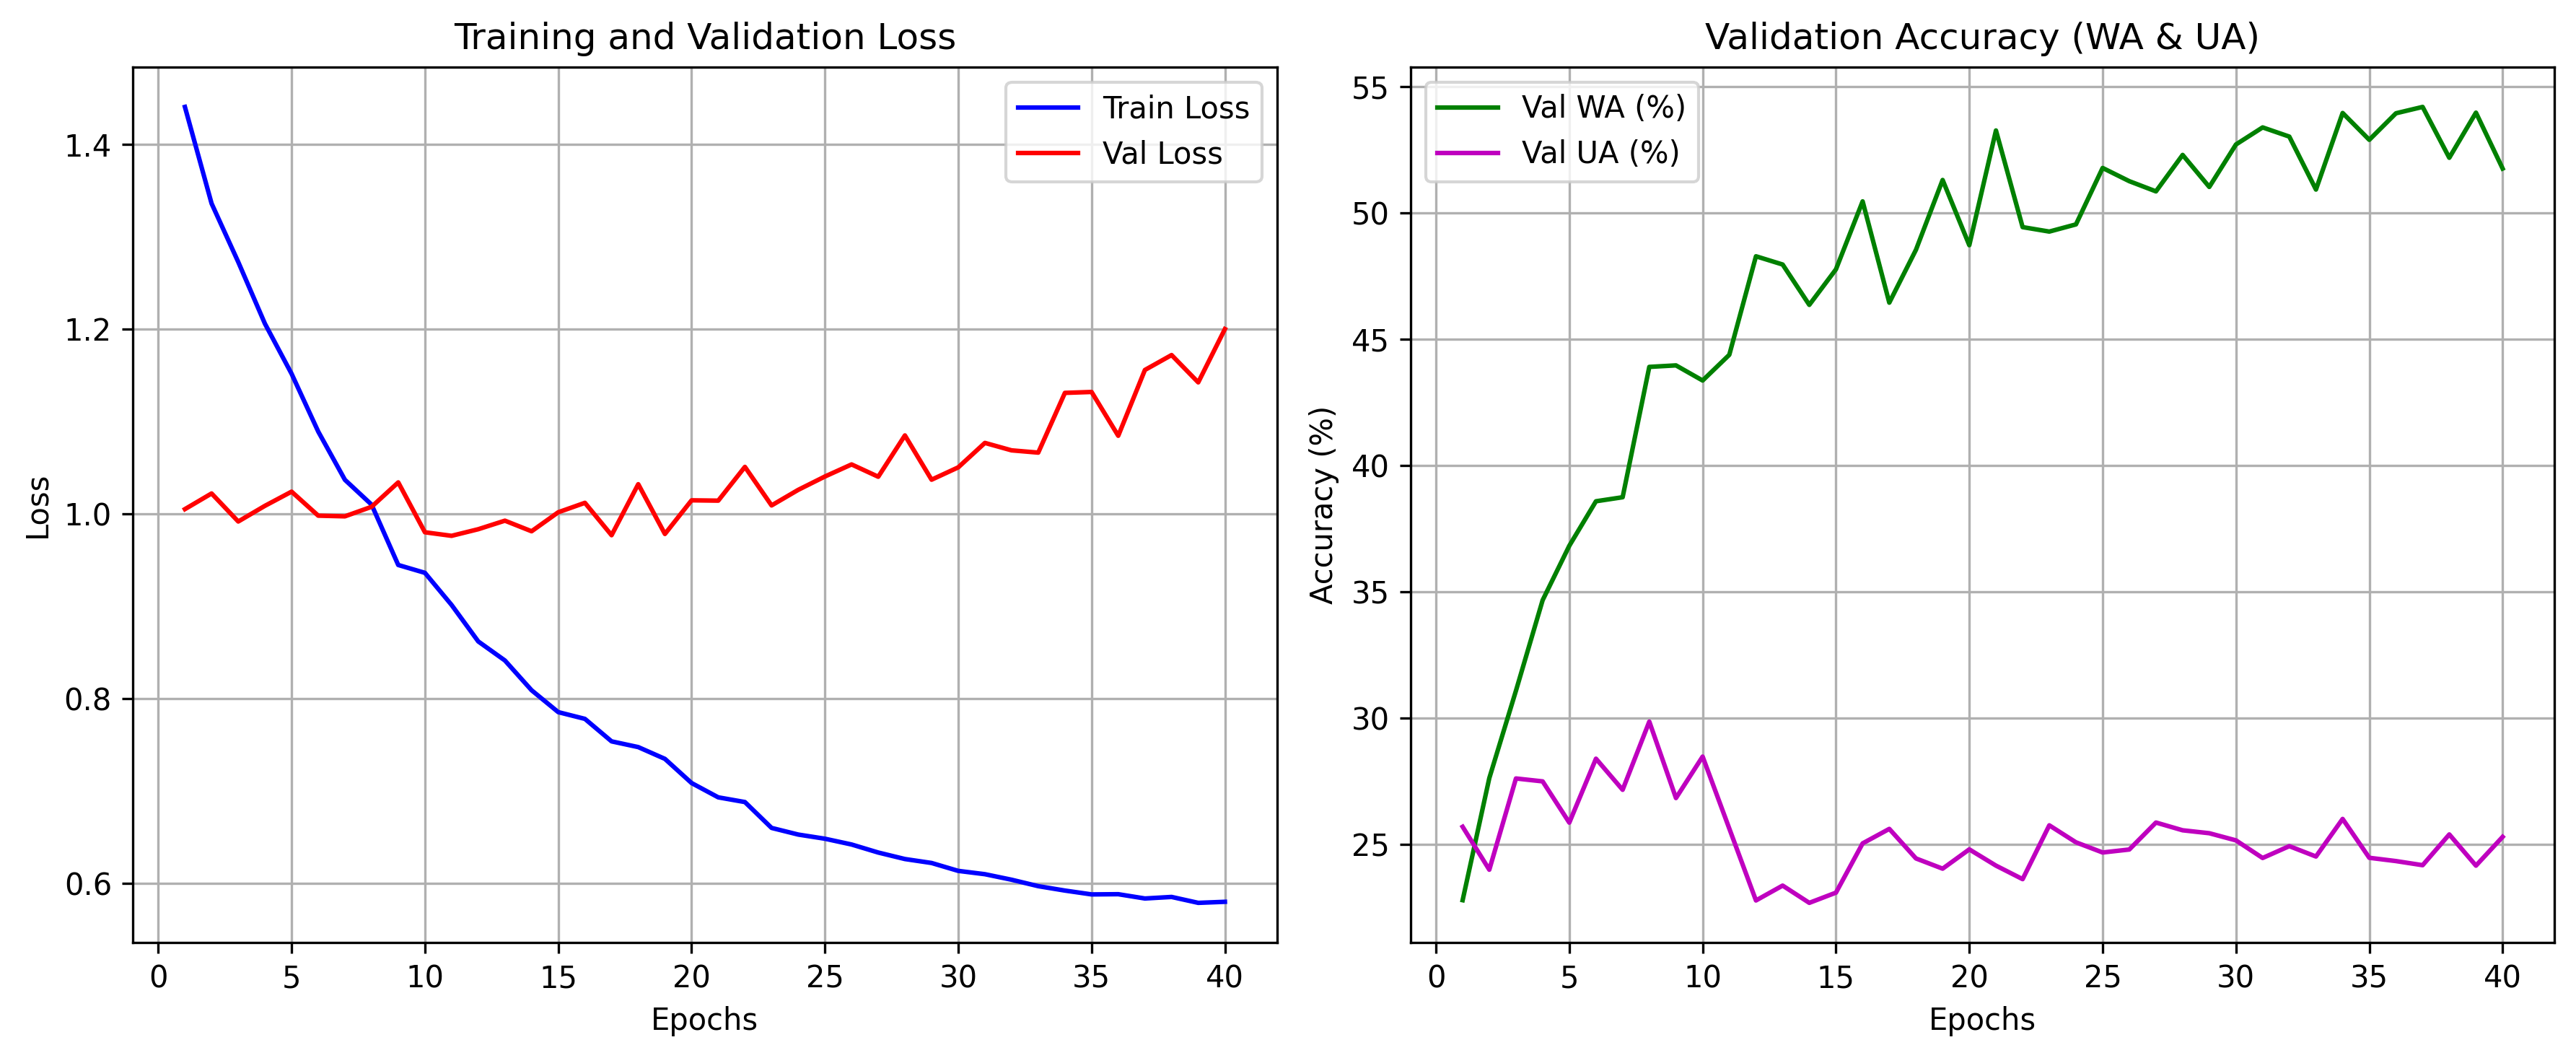
\includegraphics[width=\textwidth]{alexnet_baseline_curves.png}
        \caption{Training/Validation curves}
    \end{subfigure}
    \hfill
    \begin{subfigure}[b]{0.38\textwidth}
        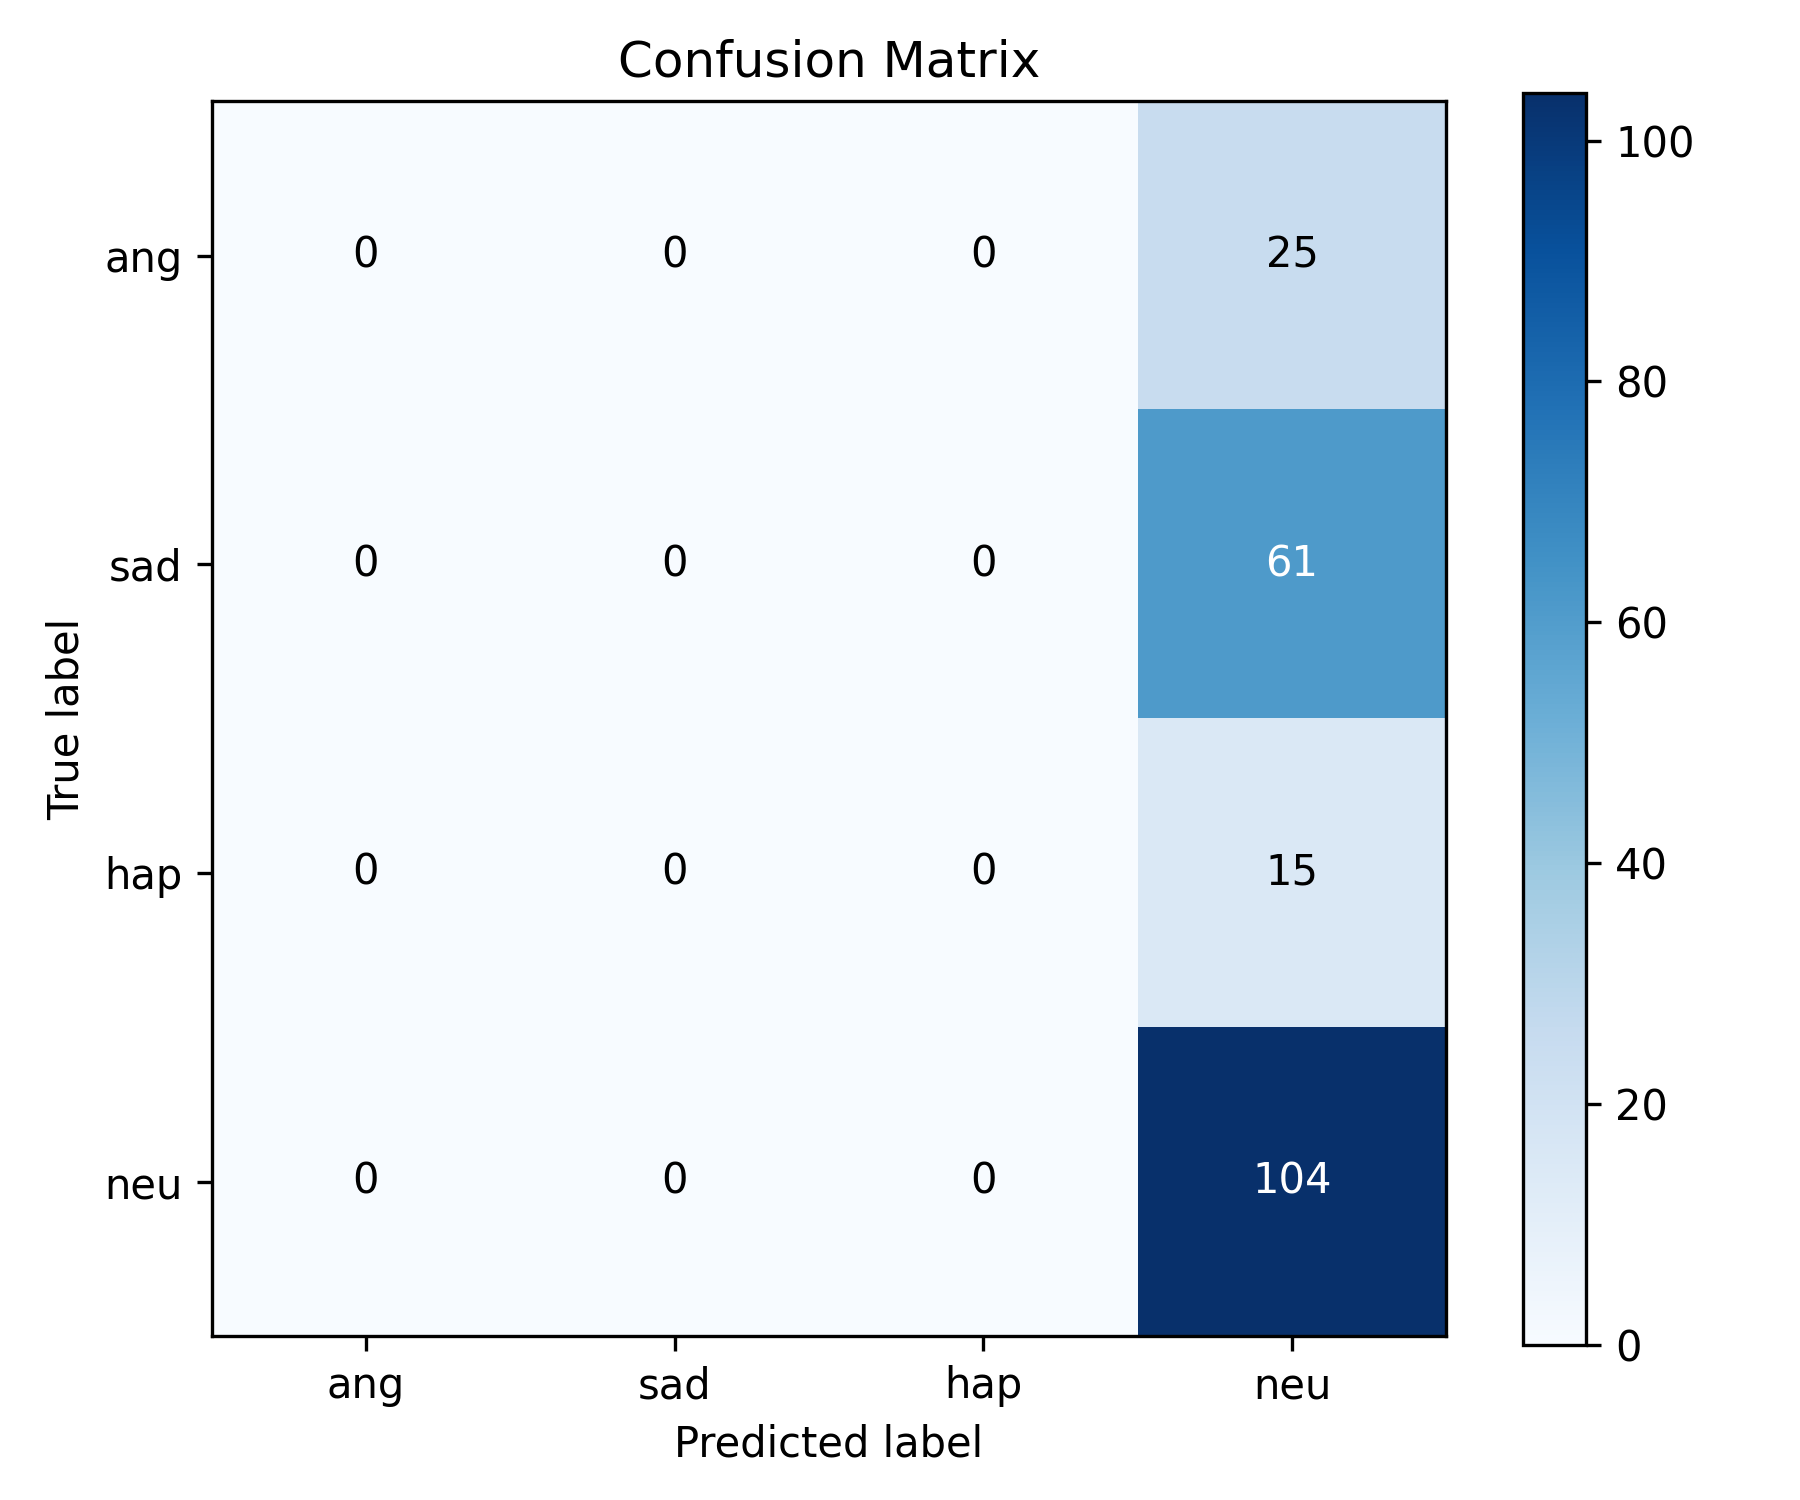
\includegraphics[width=\textwidth]{alexnet_baseline_conf.png}
        \caption{Ma trận nhầm lẫn}
    \end{subfigure}
    \caption{Kết quả AlexNet Baseline: WA=50,73\%, UA=25,00\%}
    \label{fig:alexnet_baseline}
\end{figure}

Kết quả chi tiết được minh họa trong Hình~\ref{fig:alexnet_baseline}, bao gồm đồ thị huấn luyện và ma trận nhầm lẫn của mô hình AlexNet Baseline.

Phân tích kết quả của AlexNet Baseline cho thấy mô hình bị thiên lệch hoàn toàn về phía lớp đa số (majority class bias). Mô hình phân loại toàn bộ các mẫu của tập kiểm thử vào lớp Neutral (lớp chiếm tỷ lệ lớn nhất với 50,73\% tổng số mẫu), dẫn đến độ chính xác của lớp Neutral đạt tuyệt đối 100\% trong khi cả 3 lớp còn lại (Anger, Sadness, Happiness) đều đạt 0\%. Chỉ số UA đạt đúng 25,00\% (tương đương mức dự đoán ngẫu nhiên cho 4 lớp) phản ánh rằng mô hình hoàn toàn không học được các đặc trưng phân biệt ngữ điệu giữa các cảm xúc khác nhau. Nguyên nhân chính dẫn đến hiện tượng này là do kiến trúc AlexNet nguyên bản sở hữu các lớp kết nối đầy đủ (FC) chứa lượng tham số quá lớn (57 triệu tham số) dễ gây ra hiện tượng quá khớp (overfitting) và giảm khả năng tổng quát hóa trên tập dữ liệu nhỏ. Đồng thời, hàm lỗi Cross Entropy truyền thống không thể tự điều chỉnh được ảnh hưởng của sự mất cân bằng dữ liệu cực đoan, thúc đẩy quá trình tối ưu hóa hội tụ về việc dự đoán lớp đa số Neutral nhằm giảm thiểu giá trị loss trung bình trên toàn tập dữ liệu.

\subsection{AlexNet GAP (Cross Entropy)}

\begin{figure}[H]
    \centering
    \begin{subfigure}[b]{0.55\textwidth}
        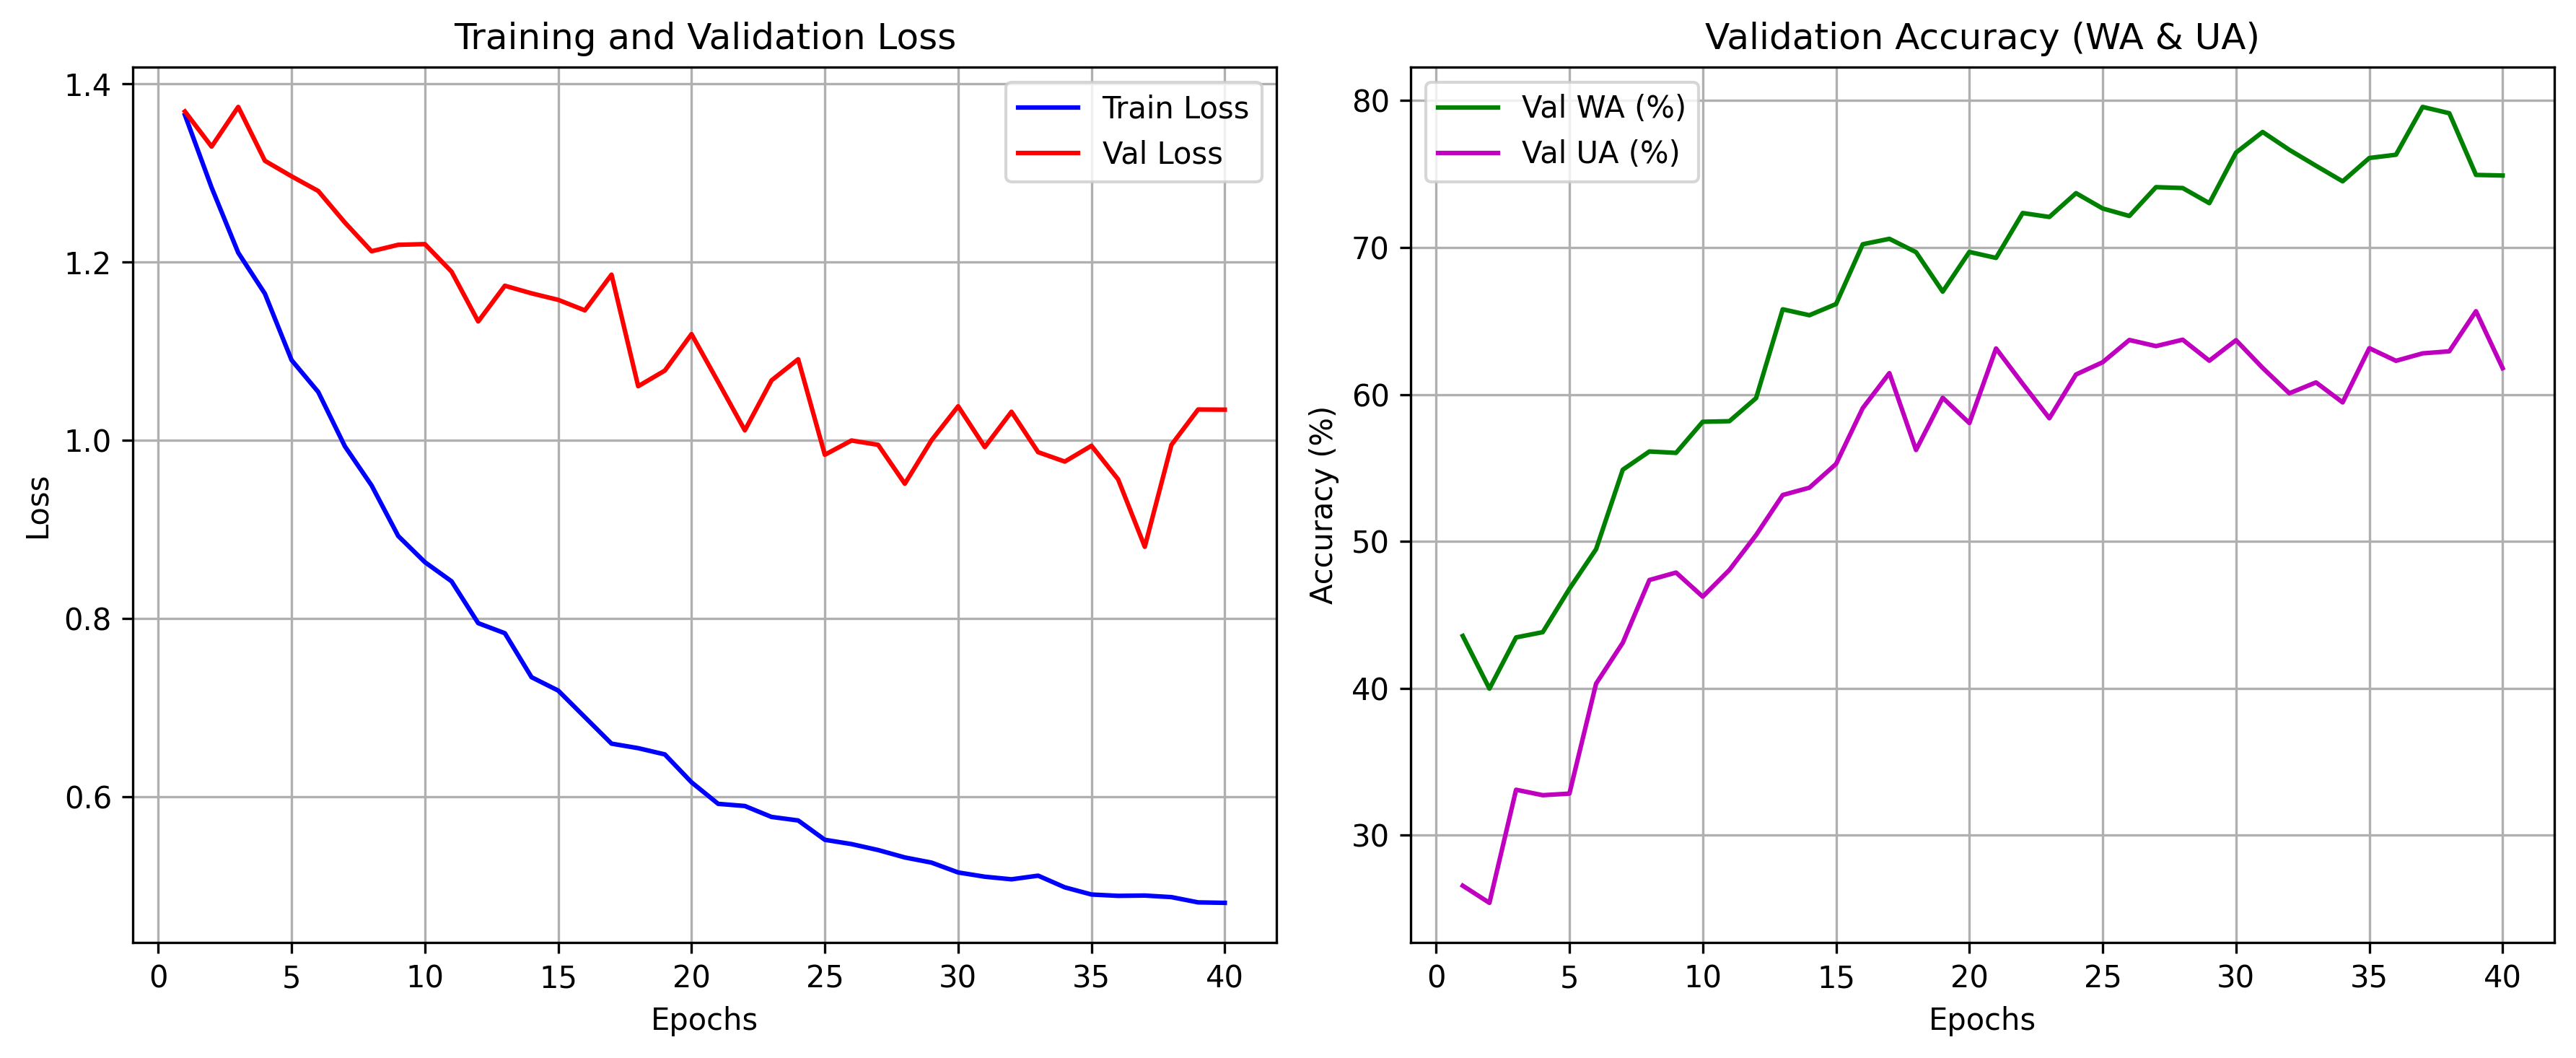
\includegraphics[width=\textwidth]{alexnet_gap_cross_entropy_curves.png}
        \caption{Training/Validation curves}
    \end{subfigure}
    \hfill
    \begin{subfigure}[b]{0.38\textwidth}
        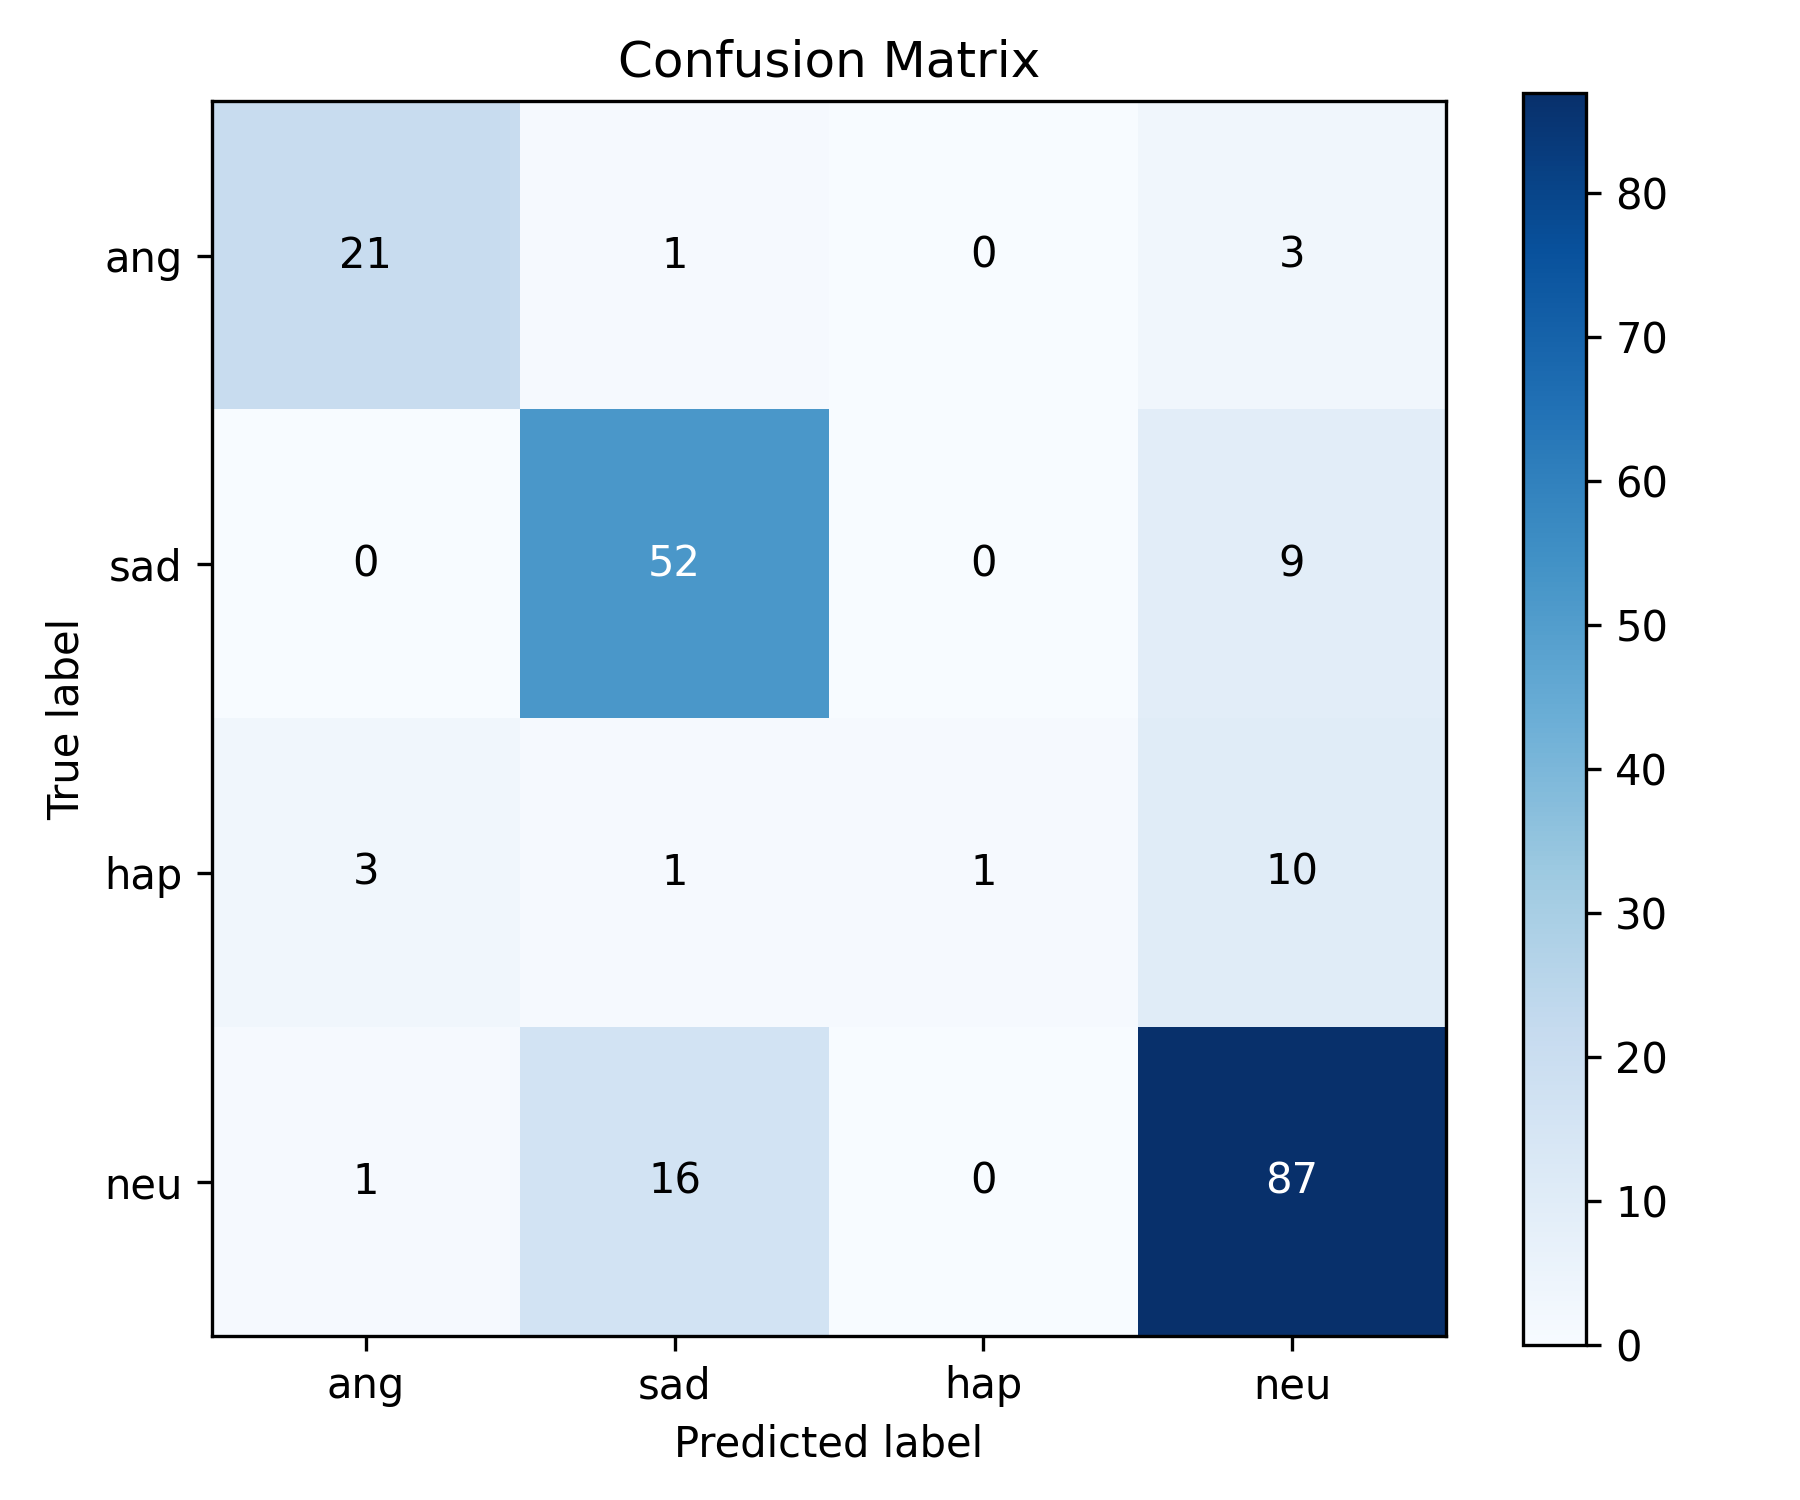
\includegraphics[width=\textwidth]{alexnet_gap_cross_entropy_conf.png}
        \caption{Ma trận nhầm lẫn}
    \end{subfigure}
    \caption{Kết quả AlexNet GAP + Cross Entropy: WA=78,54\%, UA=64,89\%}
    \label{fig:alexnet_gap}
\end{figure}

Đồ thị huấn luyện và ma trận nhầm lẫn của mô hình AlexNet GAP được minh họa trong Hình~\ref{fig:alexnet_gap}.

Đối với mô hình AlexNet GAP, việc thay thế các lớp kết nối đầy đủ bằng lớp Global Average Pooling (GAP) giúp giảm lượng tham số đến 96\% (từ 57M xuống còn 2.47M), giúp kiểm soát tốt hiện tượng quá khớp và cải thiện đáng kể Weighted Accuracy từ 50,73\% lên 78,54\% (+27,81\%). Chỉ số Unweighted Accuracy (UA) cũng tăng mạnh từ 25,00\% lên 64,89\%, chứng tỏ mô hình đã thực sự học được các đặc trưng phân biệt giữa các lớp cảm xúc thay vì đoán mò vào lớp đa số. Tuy nhiên, lớp thiểu số nhất là Happiness vẫn chỉ đạt độ chính xác ở mức thấp 38,46\%, cho thấy ảnh hưởng tiêu cực của mất cân bằng dữ liệu vẫn tồn tại khi sử dụng hàm lỗi Cross Entropy truyền thống.

\subsection{EfficientNet-B0 (Focal Loss + EMix-S) -- Mô hình tốt nhất}

\begin{figure}[H]
    \centering
    \begin{subfigure}[b]{0.55\textwidth}
        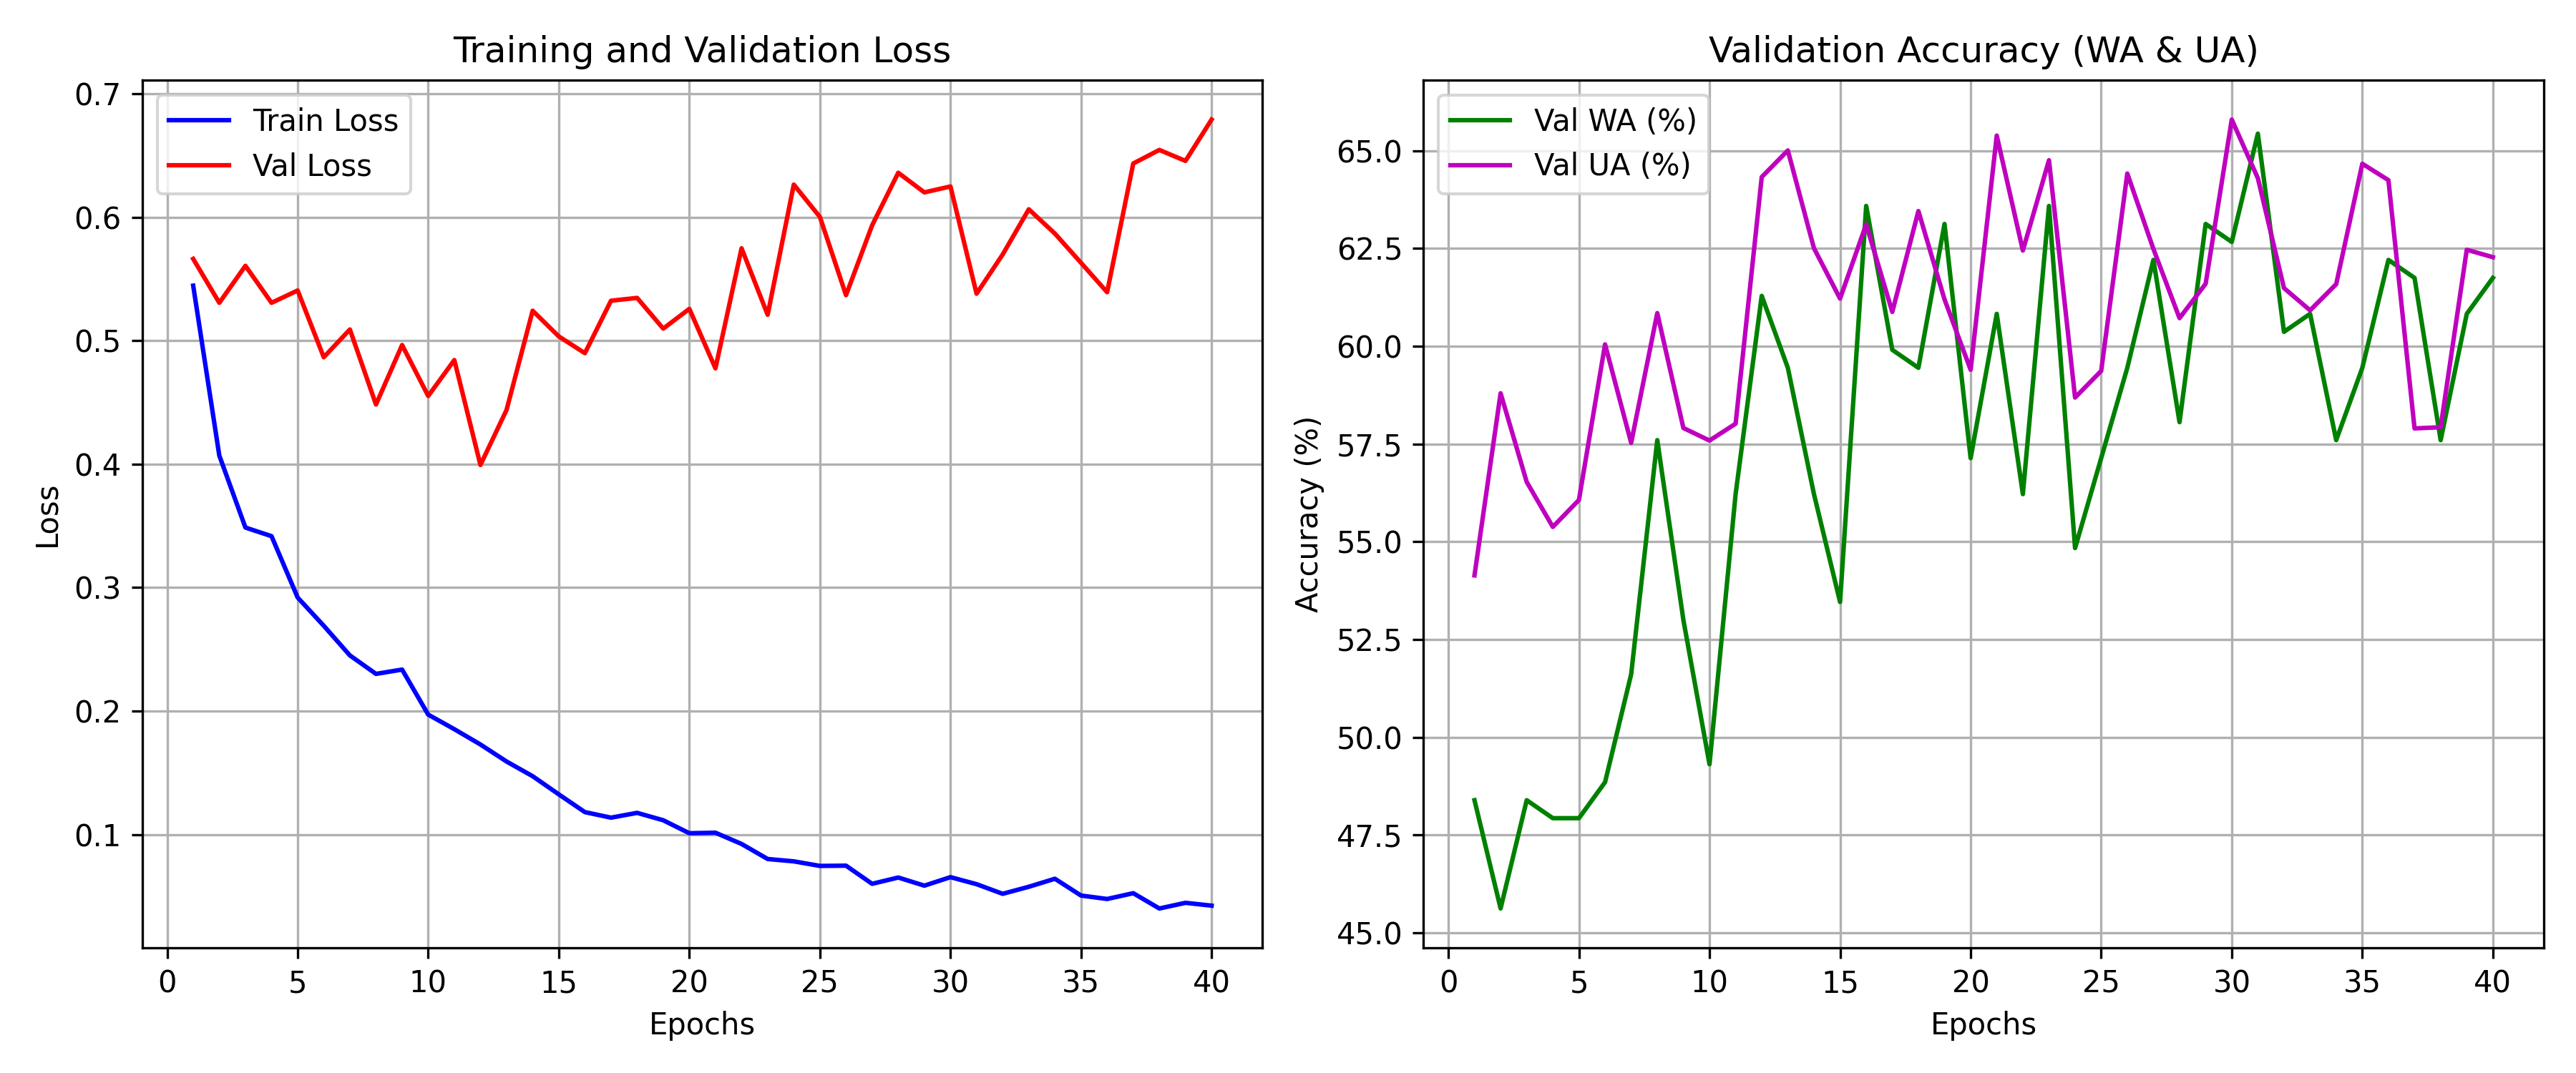
\includegraphics[width=\textwidth]{efficientnet_focal_loss_curves.png}
        \caption{Training/Validation curves}
    \end{subfigure}
    \hfill
    \begin{subfigure}[b]{0.38\textwidth}
        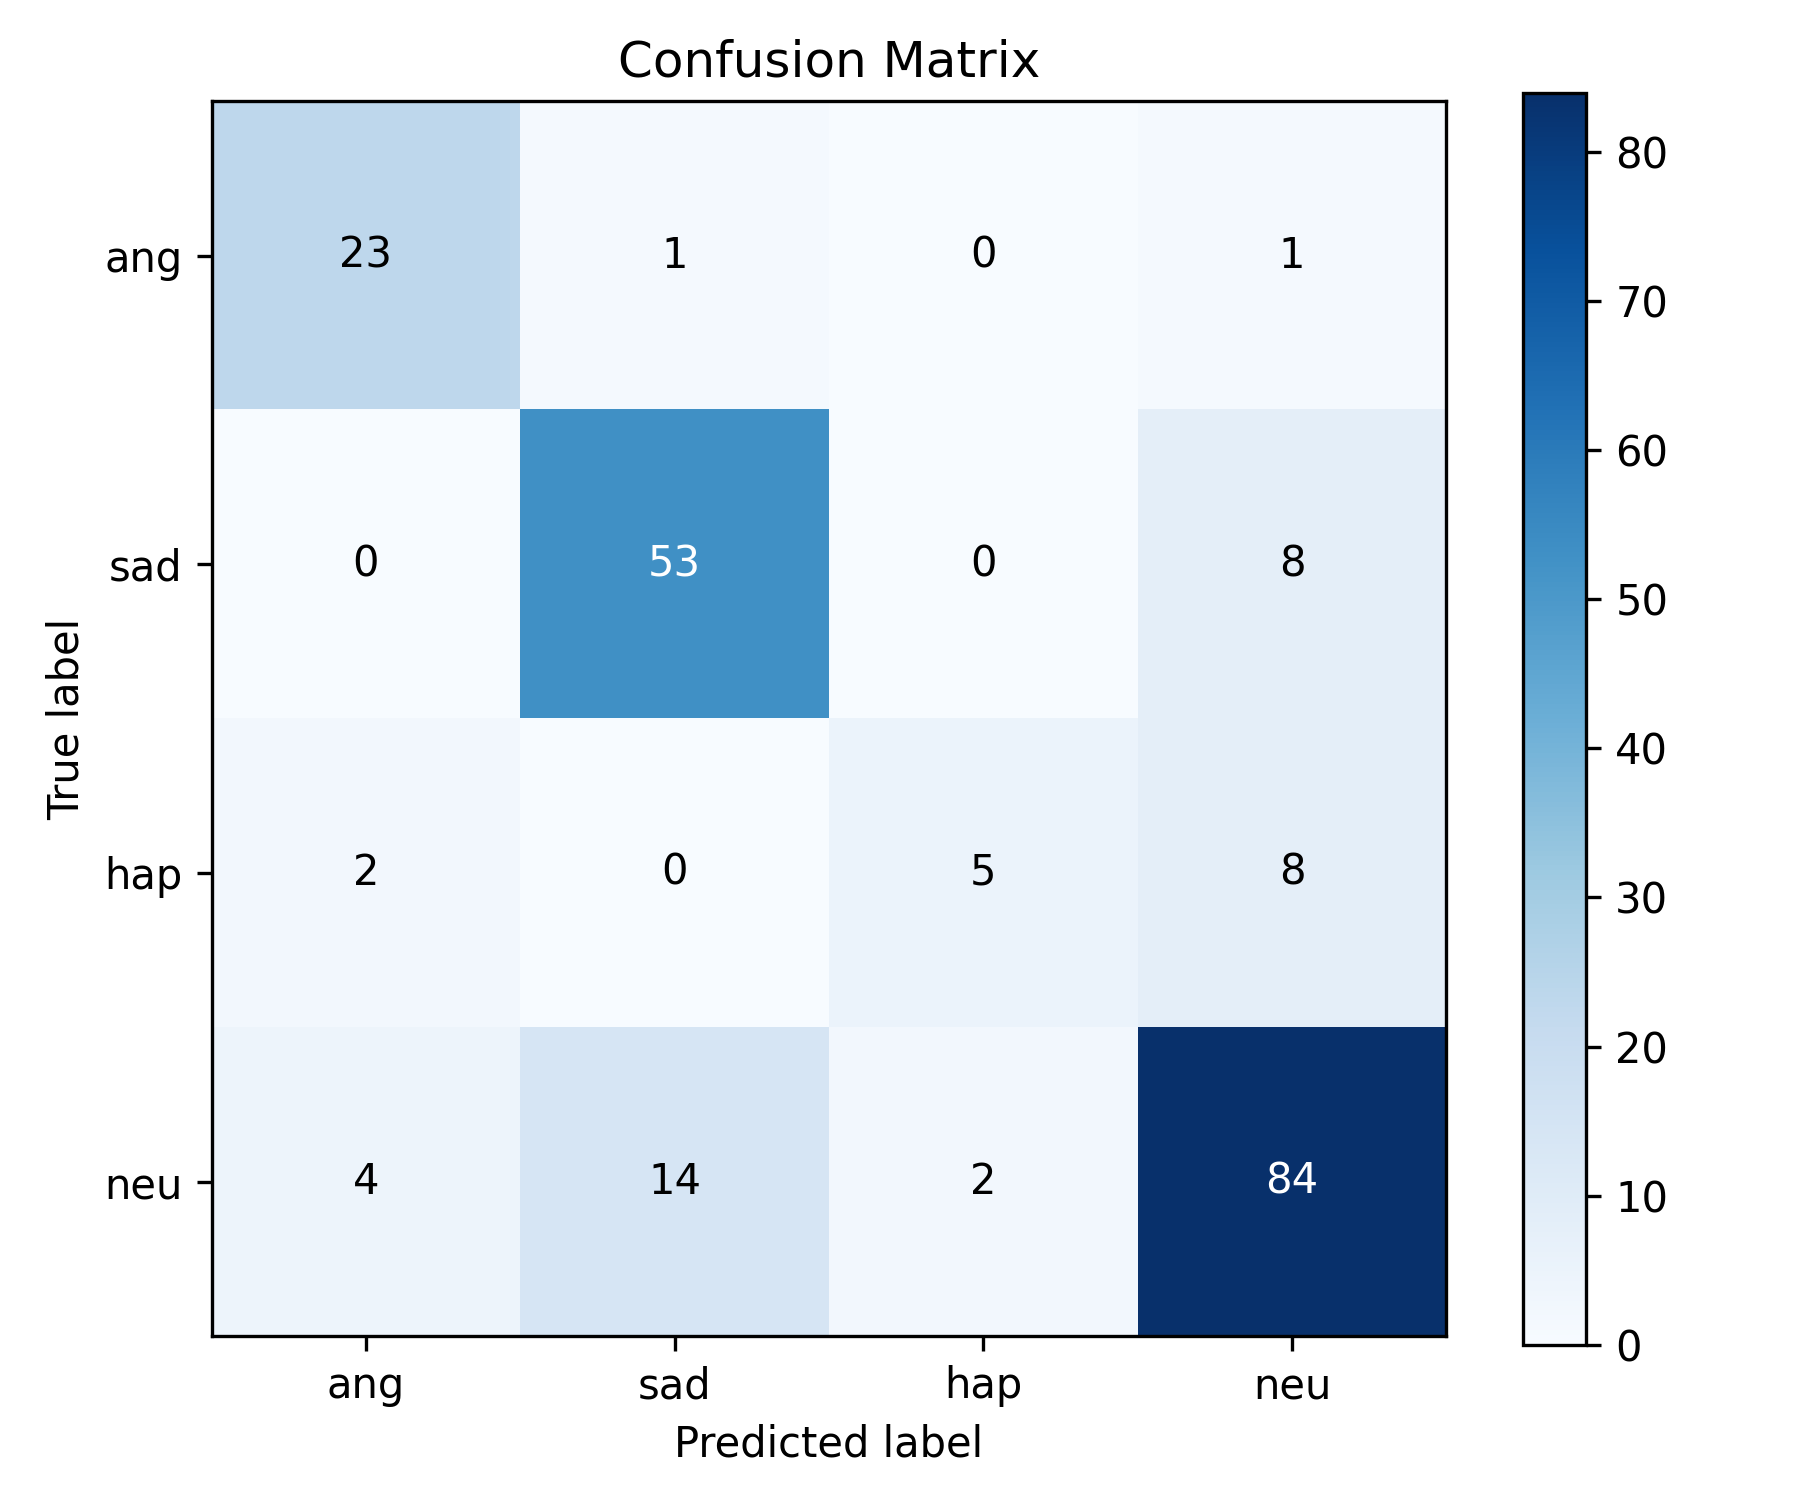
\includegraphics[width=\textwidth]{efficientnet_focal_loss_conf.png}
        \caption{Ma trận nhầm lẫn}
    \end{subfigure}
    \caption[Kết quả EfficientNet-B0 + Focal Loss + EMix-S]{Kết quả EfficientNet-B0 + Focal Loss + EMix-S: WA=80,98\%, UA=74,25\%}
    \label{fig:efficientnet_best}
\end{figure}

Đồ thị huấn luyện và ma trận nhầm lẫn của cấu hình tối ưu nhất (EfficientNet-B0 + Focal Loss + EMix-S) được trình bày tại Hình~\ref{fig:efficientnet_best}.

Mô hình EfficientNet-B0 kết hợp Focal Loss và EMix-S đạt hiệu năng tối ưu nhất trên tập kiểm thử với chỉ số WA đạt 80,98\% và UA đạt 74,25\%. Chỉ sở hữu 4,01 triệu tham số (tương đương 7\% kích thước của AlexNet gốc), mô hình mang lại hiệu suất vượt trội nhờ cơ chế Compound Scaling. Độ chính xác trên lớp thiểu số nhất Happiness được cải thiện vượt bậc từ 0,00\% ở cấu hình baseline lên mức 61,54\%. Tuy nhiên, do ba yếu tố thay đổi đồng thời bao gồm kiến trúc mạng, hàm lỗi và phương pháp tăng cường dữ liệu, mức cải thiện tổng thể này là kết quả cộng hưởng của nhiều yếu tố và không thể quy riêng cho một thành phần đơn lẻ. Phân tích chi tiết đóng góp của từng thành phần được trình bày tại Mục~\ref{sec:ablation}. Mô hình này đạt giá trị Test Loss thấp nhất ở mức 0,2792, khẳng định khả năng tổng quát hóa tốt nhất trên phân bố dữ liệu kiểm thử.

\subsection{Các mô hình khác}

\begin{figure}[H]
    \centering
    \begin{subfigure}[b]{0.48\textwidth}
        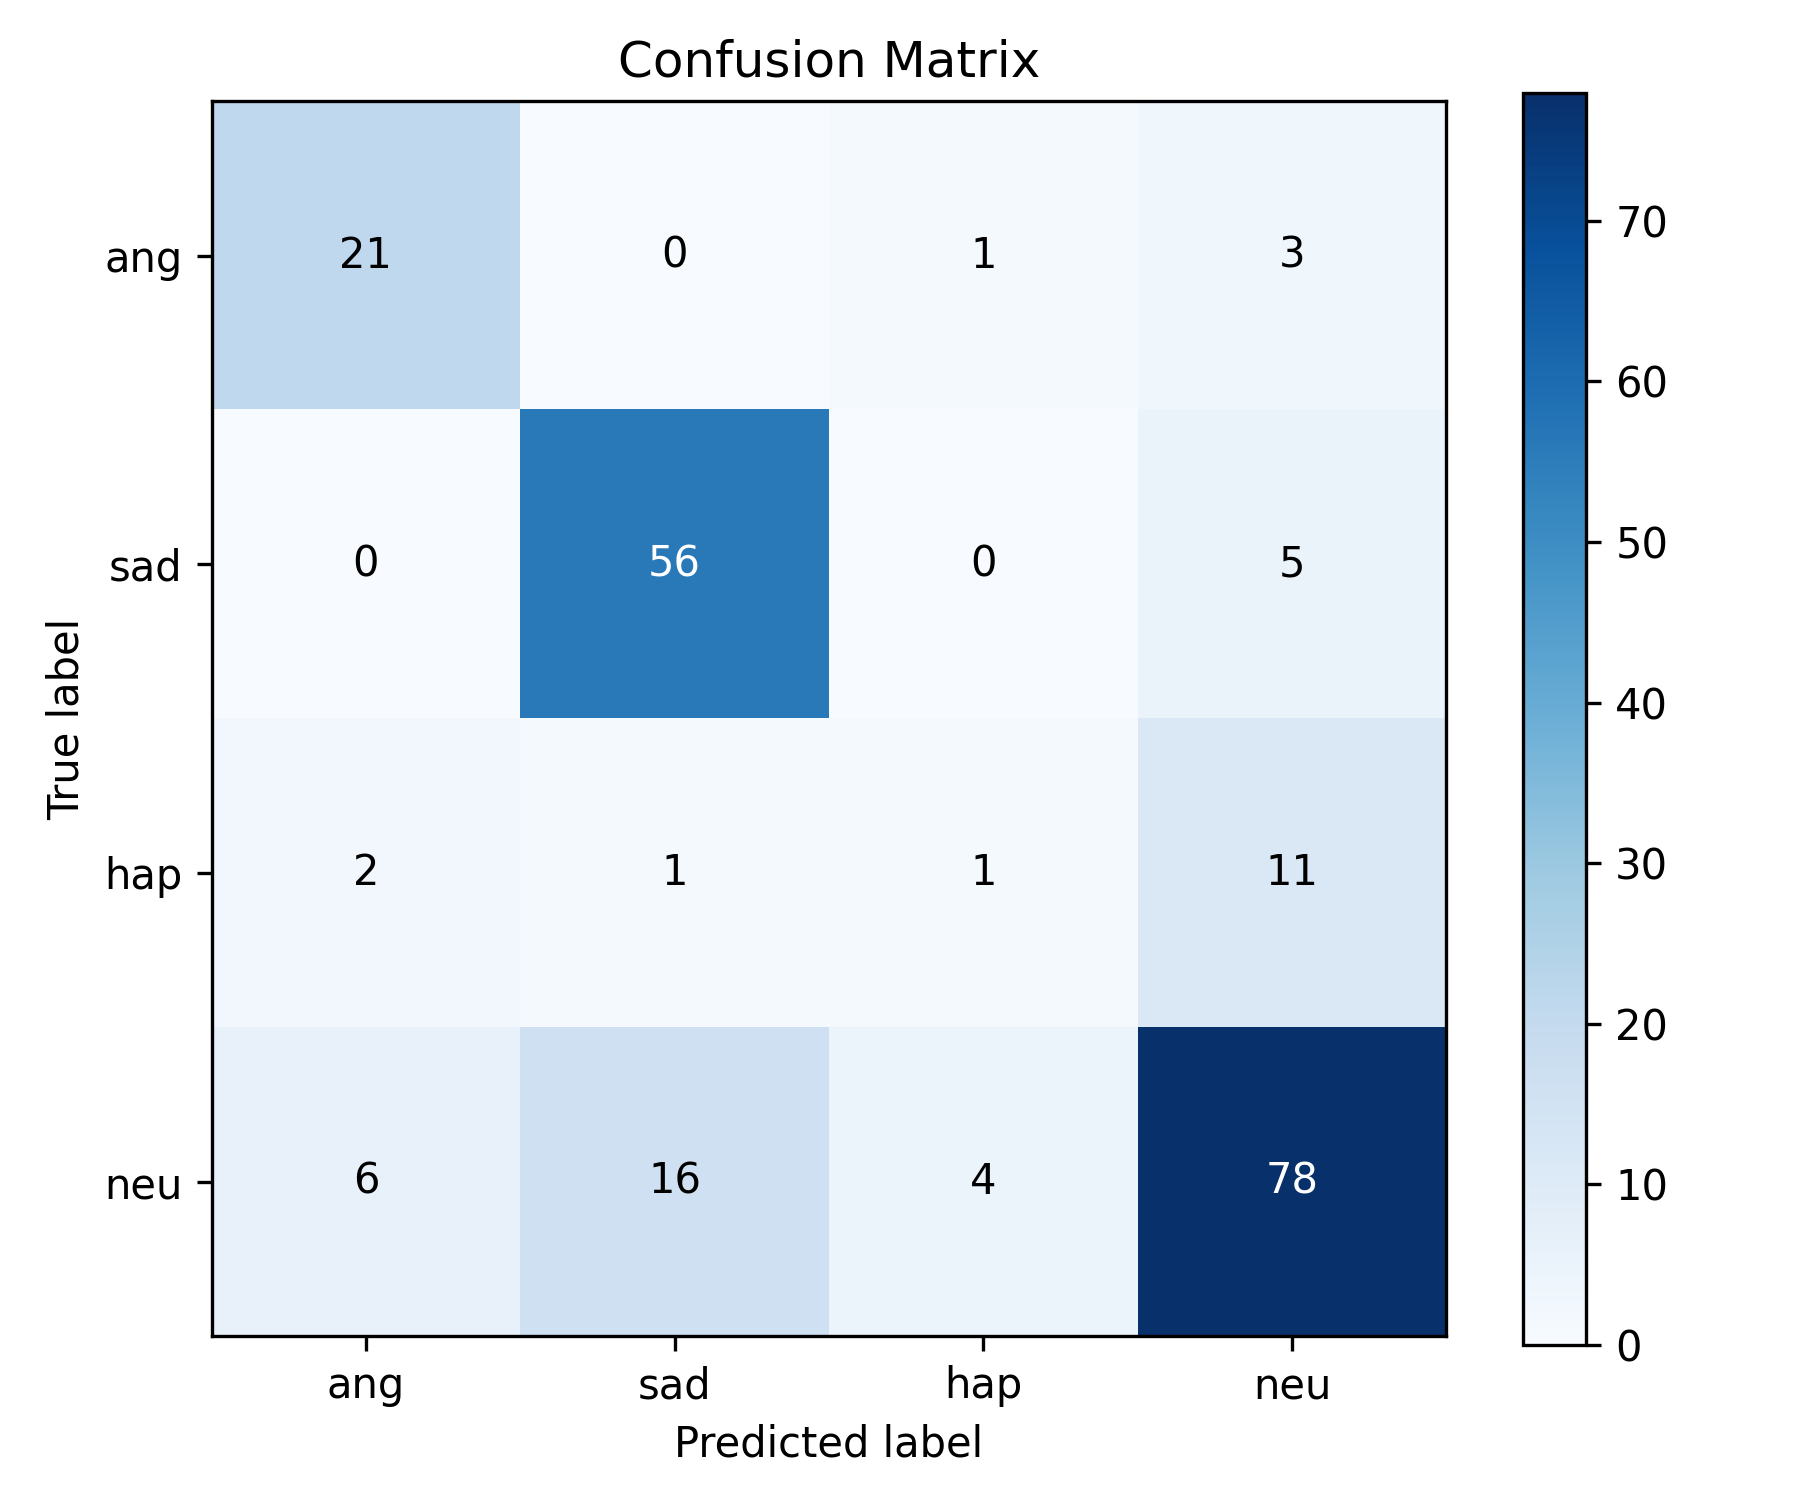
\includegraphics[width=\textwidth]{resnet_focal_loss_conf.png}
        \caption{ResNet-18: WA=76,10\%, UA=64,37\%}
    \end{subfigure}
    \hfill
    \begin{subfigure}[b]{0.48\textwidth}
        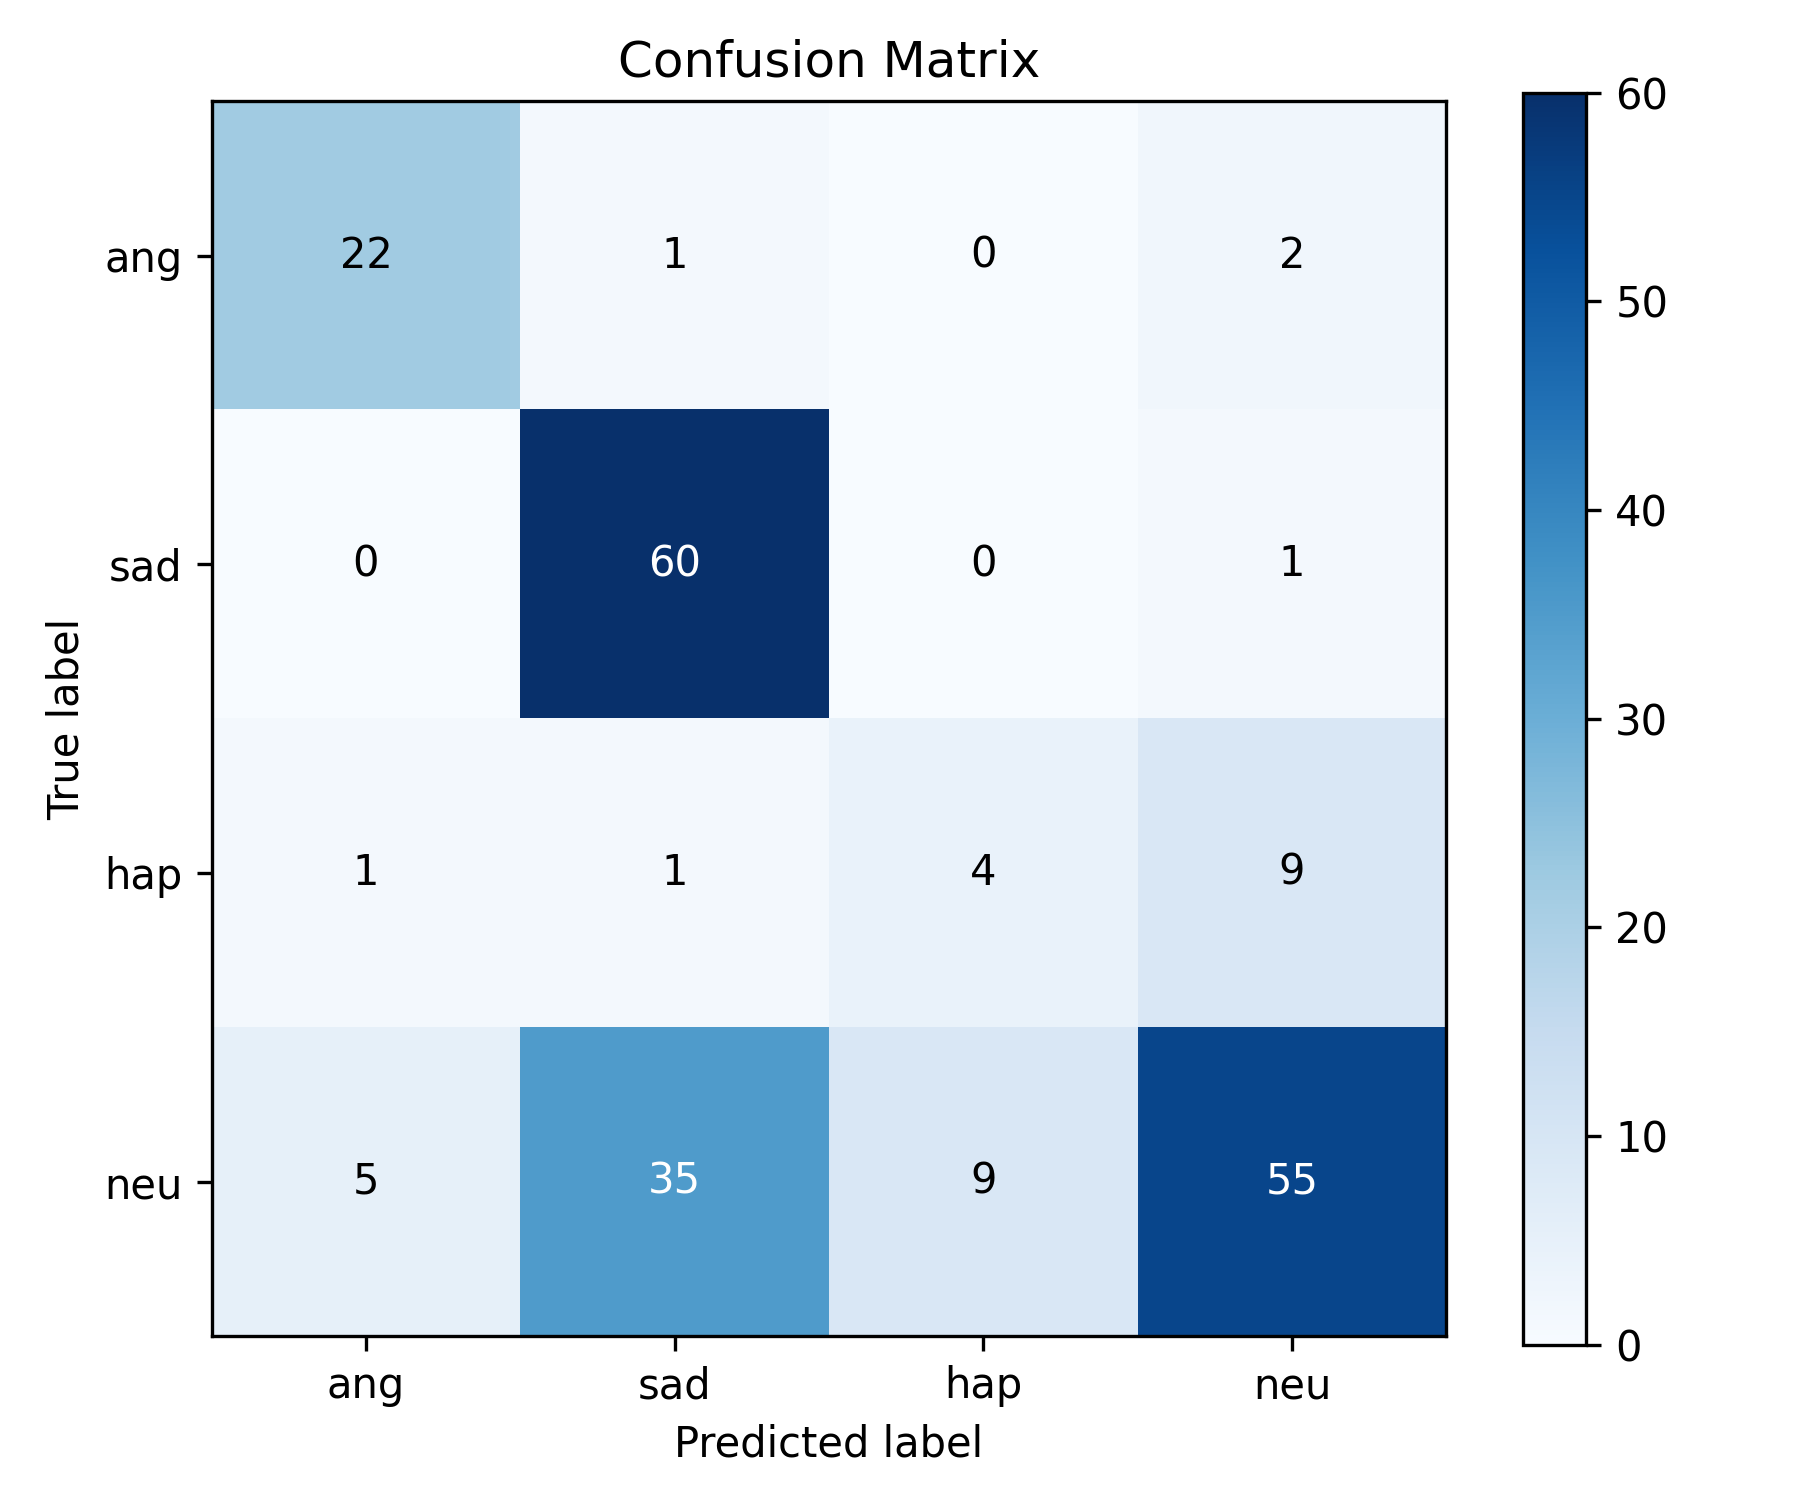
\includegraphics[width=\textwidth]{densenet_focal_loss_conf.png}
        \caption{DenseNet-121: WA=68,78\%, UA=66,48\%}
    \end{subfigure}
    \\[0.5cm]
    \begin{subfigure}[b]{0.48\textwidth}
        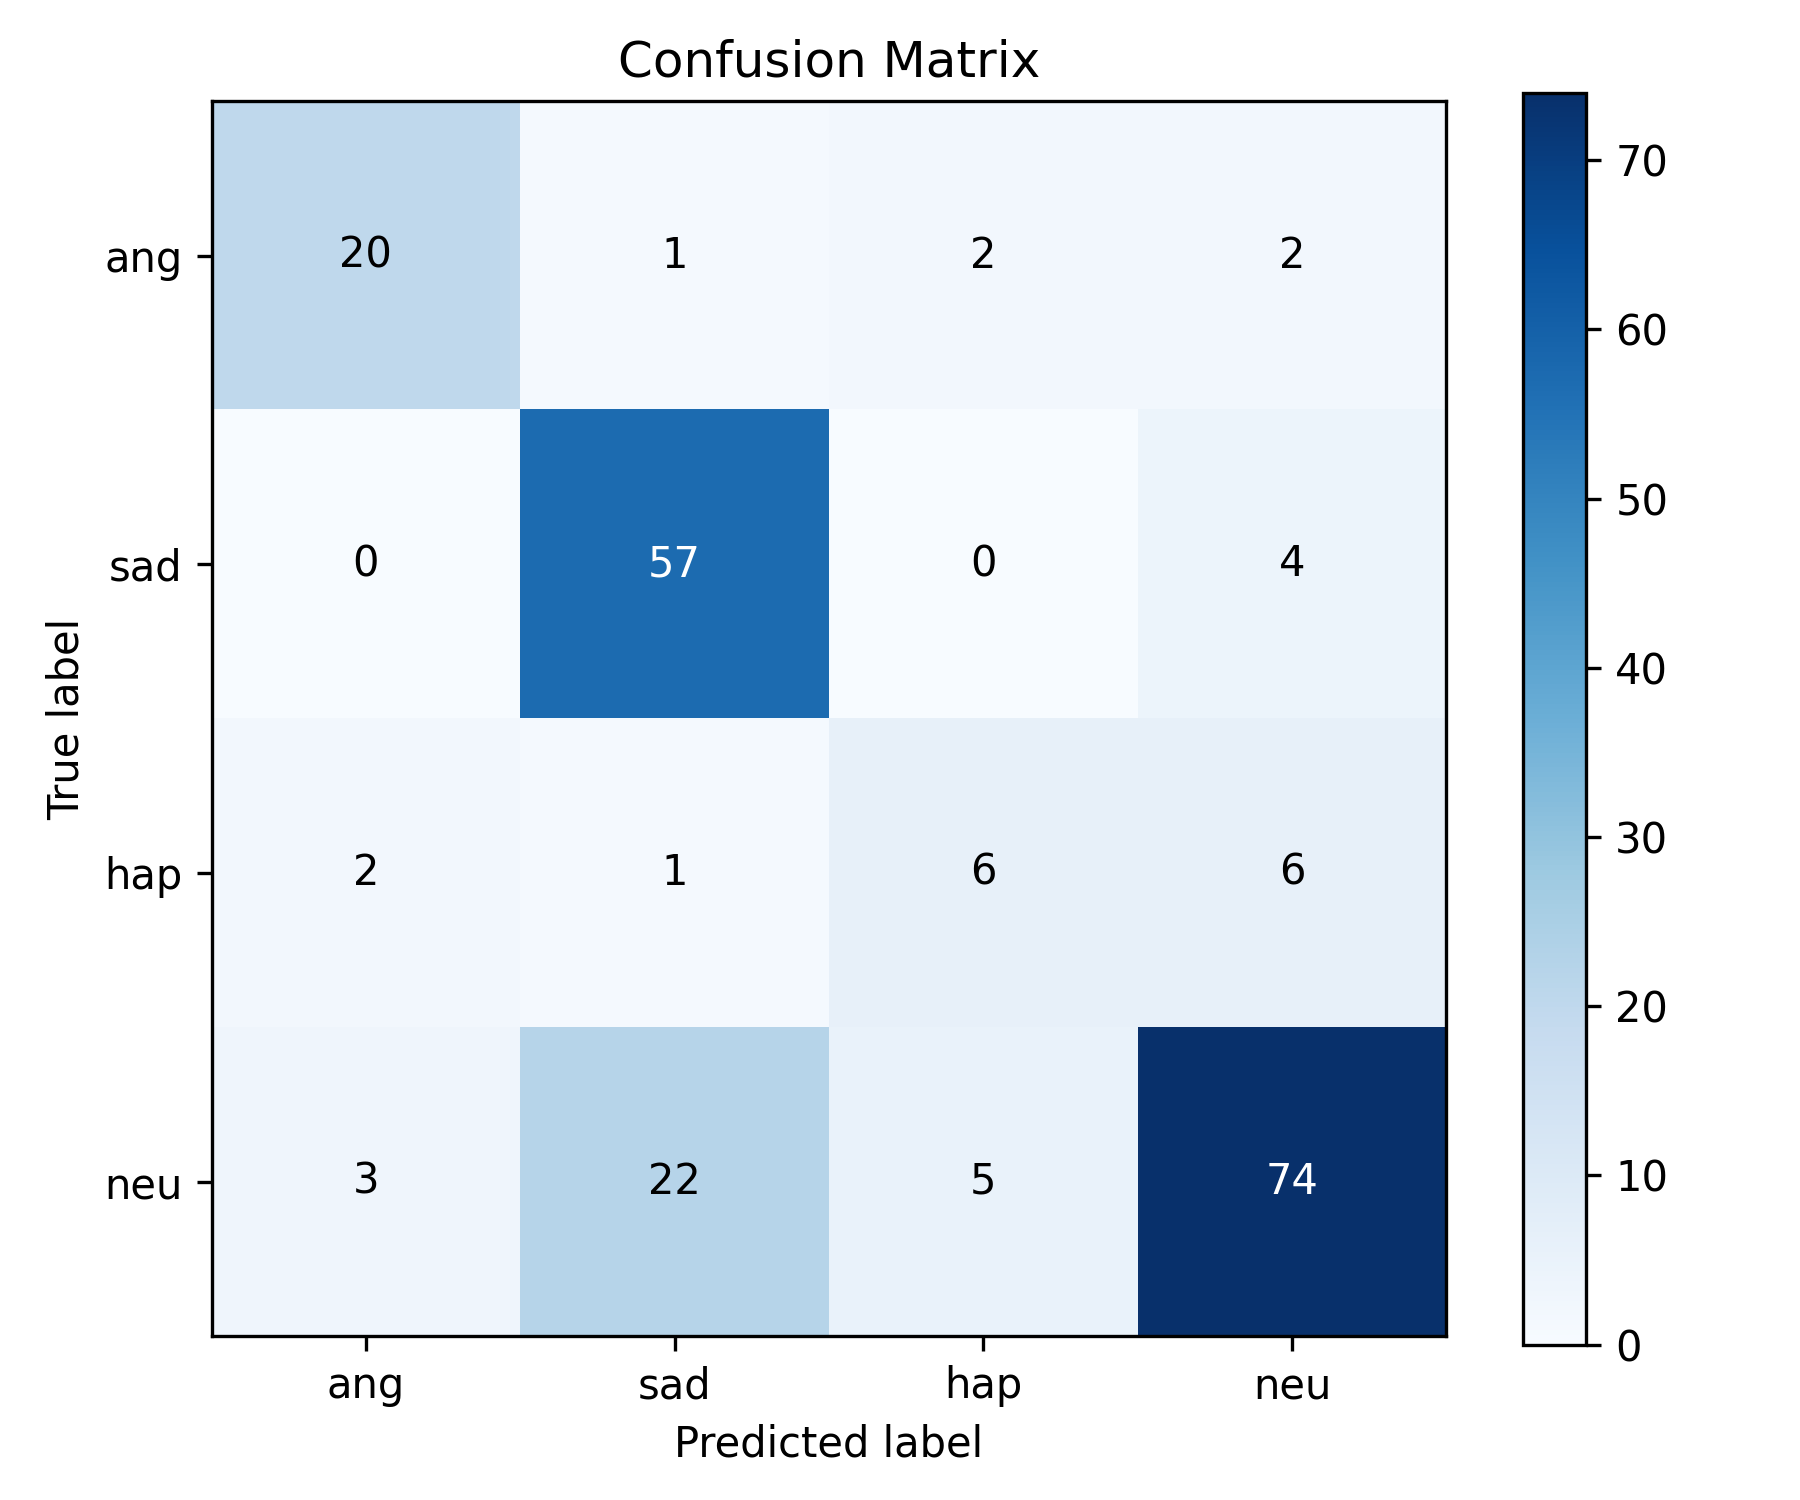
\includegraphics[width=\textwidth]{mobilenet_focal_loss_conf.png}
        \caption{MobileNet-V2: WA=76,59\%, UA=71,15\%}
    \end{subfigure}
    \caption[Ma trận nhầm lẫn của các mô hình khác]{Ma trận nhầm lẫn của các mô hình ResNet-18, DenseNet-121 và MobileNet-V2}
    \label{fig:other_models}
\end{figure}

Ma trận nhầm lẫn chi tiết của các mô hình ResNet-18, DenseNet-121 và MobileNet-V2 được thể hiện tương ứng trong Hình~\ref{fig:other_models}. Qua đó, MobileNet-V2 chứng minh hiệu quả tốt thứ hai với UA đạt 71,15\% nhờ sử dụng các khối nghịch đảo Inverted Residuals và Linear Bottlenecks giúp giữ thông tin ngữ điệu hiệu quả.


\section{Phân tích Per-class Accuracy}
\label{sec:per_class}

Bảng~\ref{tab:per_class} trình bày độ chính xác phân loại theo từng nhãn cảm xúc cho tất cả các mô hình.

\begin{table}[H]
\centering
\caption{Độ chính xác theo từng nhãn cảm xúc (\%)}
\label{tab:per_class}
\begin{tabular}{lccccc}
\toprule
\textbf{Mô hình} & \textbf{Anger} & \textbf{Sadness} & \textbf{Happiness} & \textbf{Neutral} & \textbf{UA (\%)} \\
\midrule
AlexNet (Baseline) & 0,00 & 0,00 & 0,00 & 100,00 & 25,00 \\
AlexNet GAP & 84,62 & 56,41 & 38,46 & 80,08 & 64,89 \\
ResNet-18 & 84,62 & 53,85 & 38,46 & 80,62 & 64,37 \\
DenseNet-121 & 69,23 & 61,54 & 53,85 & 81,30 & 66,48 \\
\textbf{EfficientNet-B0} $\star$ & \textbf{92,31} & 61,54 & \textbf{61,54} & 77,62 & \textbf{73,25} \\
MobileNet-V2 & 84,62 & 64,10 & 53,85 & 81,99 & 71,15 \\
\bottomrule
\end{tabular}
\end{table}

\begin{figure}[H]
    \centering
    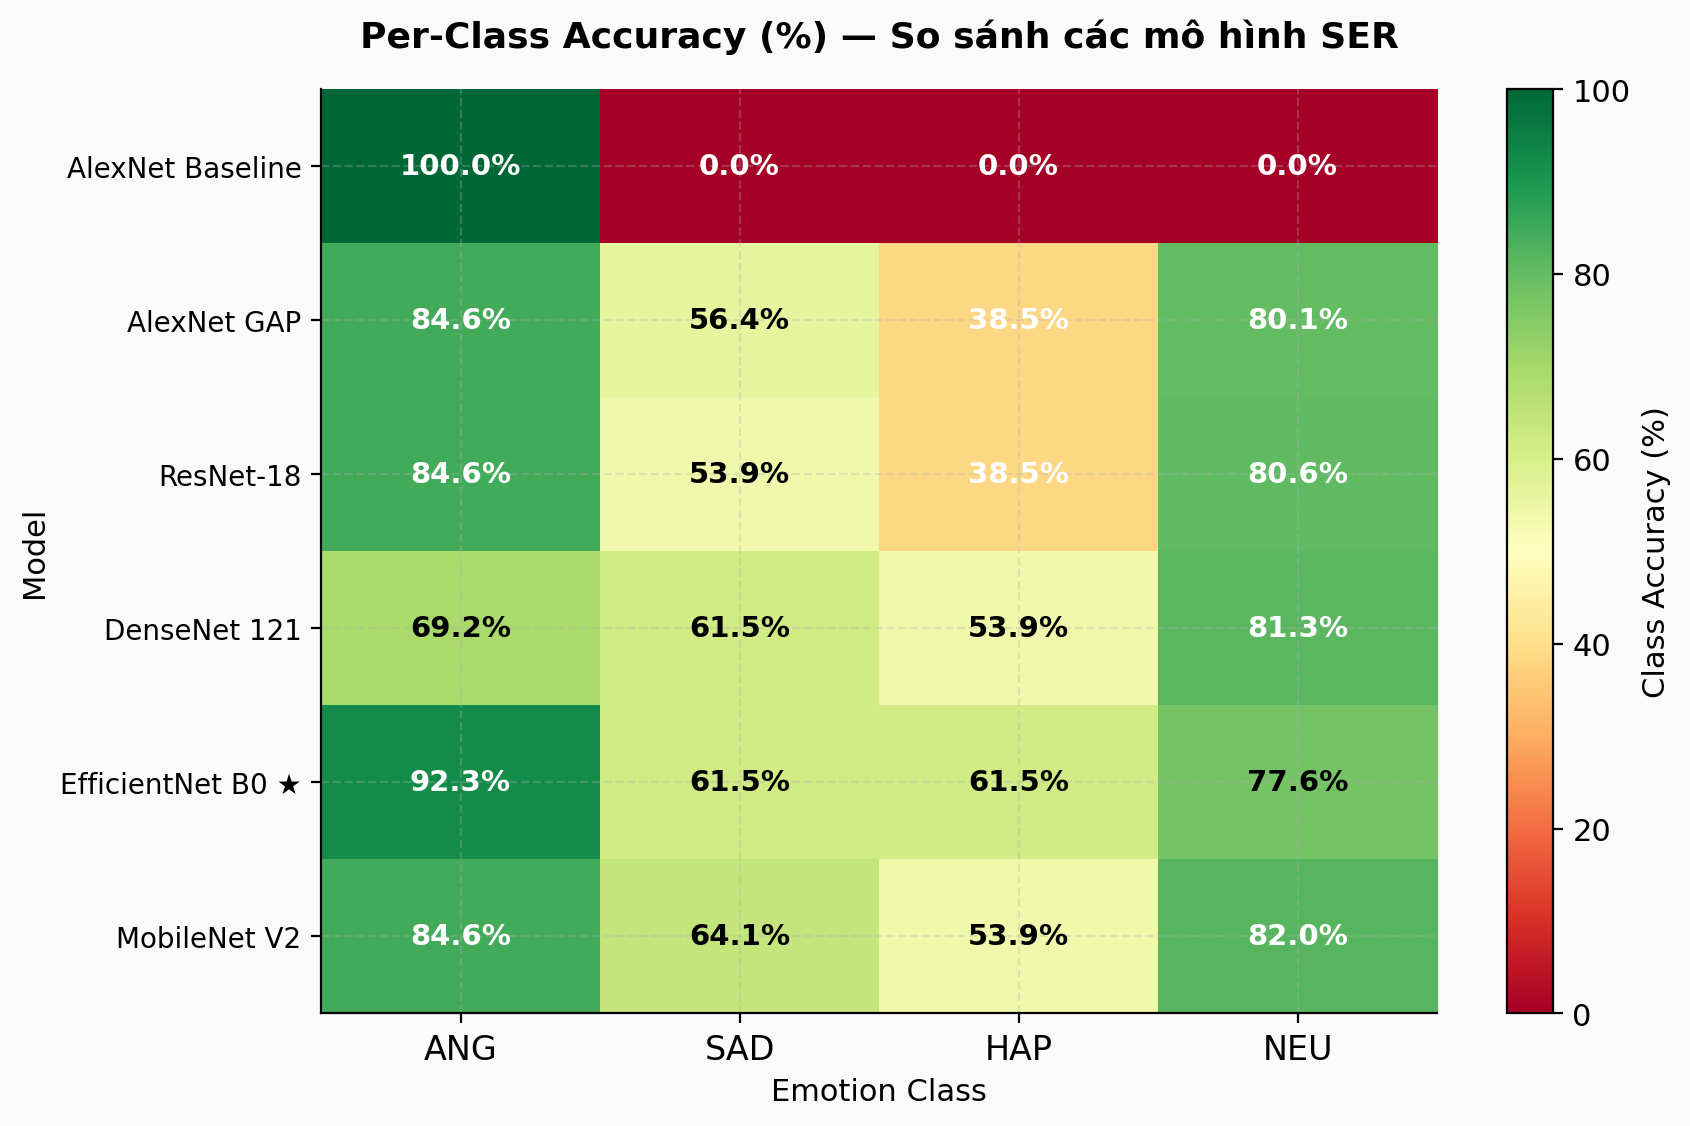
\includegraphics[width=0.85\textwidth]{comparison_per_class.png}
    \caption{Heatmap so sánh per-class accuracy giữa các mô hình}
    \label{fig:per_class_heatmap}
\end{figure}

Bảng~\ref{tab:per_class} liệt kê chi tiết kết quả. Biểu đồ heatmap so sánh độ chính xác theo từng lớp được trực quan hóa tại Hình~\ref{fig:per_class_heatmap}.

Phân tích chi tiết độ chính xác theo từng lớp cảm xúc chỉ ra các đặc tính học của mô hình. Đối với lớp đa số Neutral, mặc dù mô hình baseline đạt 100\% nhưng đó hoàn toàn là do thiên lệch lớp, trong khi EfficientNet-B0 duy trì độ chính xác cao ổn định ở mức 77,62\% mà không bị thiên lệch. Ở lớp Anger, EfficientNet-B0 đạt độ chính xác cao nhất với 92,31\%, cải thiện vượt trội so với mức 0,00\% của Baseline, chứng minh mô hình đã học được các đặc trưng biên độ lớn của cảm xúc tức giận. Đối với lớp thiểu số nhất Happiness, độ chính xác được cải thiện vượt bậc từ 0,00\% (Baseline) lên 61,54\% (EfficientNet-B0), chứng minh hiệu quả thực tế của Focal Loss kết hợp tăng cường dữ liệu EMix-S trong việc giải quyết vấn đề mất cân bằng dữ liệu cực đoan. Lớp Sadness đạt mức độ chính xác 61,54\% đối với EfficientNet-B0 và tiếp tục là một trong những lớp khó phân loại nhất do có sự tương đồng đặc trưng âm học rất lớn với lớp Neutral (cùng thuộc nhóm arousal thấp: cao độ thấp, năng lượng âm thanh yếu và tốc độ phát âm chậm).


\section{Ablation Study}
\label{sec:ablation}

Để đánh giá đóng góp riêng lẻ của từng kỹ thuật cải tiến, thực nghiệm Ablation Study được thực hiện trên EfficientNet-B0 với các cấu hình kết quả cụ thể trên tập kiểm thử được trình bày trong Bảng~\ref{tab:ablation}.

\begin{table}[H]
\centering
\caption{Kết quả Ablation Study -- EfficientNet-B0}
\label{tab:ablation}
\begin{tabular}{clllrr}
\toprule
\textbf{Config} & \textbf{Mô hình} & \textbf{Loss} & \textbf{Augmentation} & \textbf{WA (\%)} & \textbf{UA (\%)} \\
\midrule
A & EfficientNet-B0 & Cross Entropy & Không & 74,15 & 58,46 \\
B & EfficientNet-B0 & Focal Loss & Không & 77,07 & 66,83 \\
\textbf{C} & \textbf{EfficientNet-B0} & \textbf{Focal Loss} & \textbf{EMix-S} & \textbf{80,98} & \textbf{74,25} \\
D & EfficientNet-B0 & Focal Loss & EMix-NS & 78,54 & 70,98 \\
\bottomrule
\end{tabular}
\end{table}

Ma trận nhầm lẫn của cấu hình cơ sở (Config A) được thể hiện tại Hình~\ref{fig:ablation_ce}.

\begin{figure}[H]
    \centering
    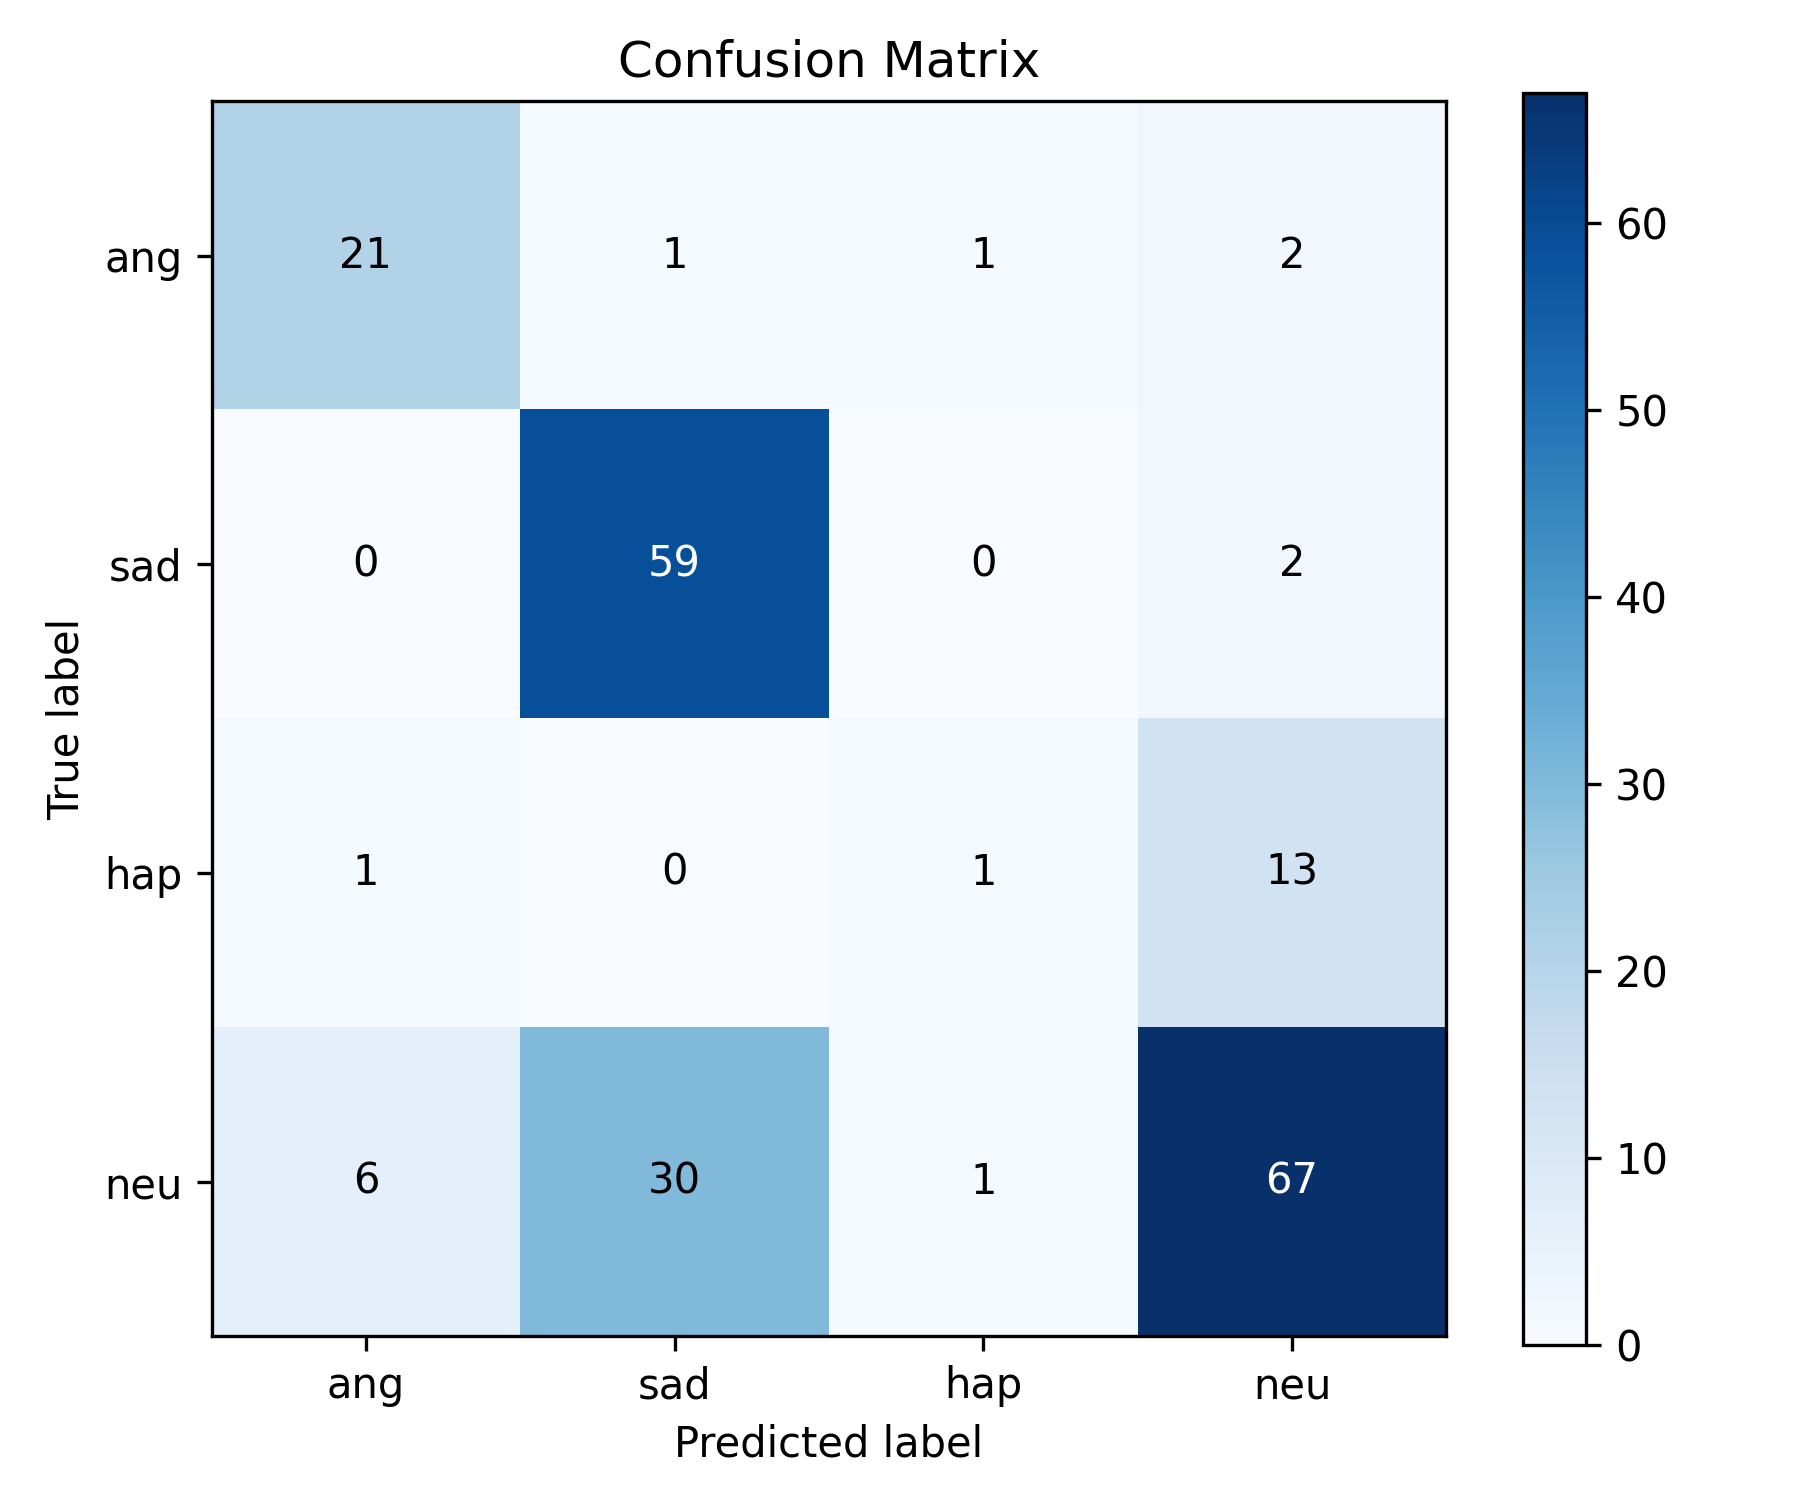
\includegraphics[width=0.42\textwidth]{efficientnet_ce_no_emix_conf.png}
    \caption{Ma trận nhầm lẫn của cấu hình cơ sở (Config A: EfficientNet-B0 + CE)}
    \label{fig:ablation_ce}
\end{figure}

Phân tích kết quả thực nghiệm Ablation Study chỉ ra đóng góp riêng lẻ của từng cấu phần. Khi chuyển đổi từ cấu hình cơ sở sang sử dụng Focal Loss (Config A sang Config B), chỉ số WA tăng từ 74,15\% lên 77,07\% (+2,92\%) và UA tăng vượt bậc từ 58,46\% lên 66,83\% (+8,37\%), chứng minh hiệu năng rõ rệt của Focal Loss trong việc giải quyết mất cân bằng dữ liệu bằng cách tập trung vào các mẫu khó. Tiếp theo, việc tích hợp thêm kỹ thuật tăng cường dữ liệu EMix-S (Config B sang Config C) giúp WA tăng thêm 3,91\% (đạt 80,98\%) và UA tăng thêm 7,42\% (đạt 74,25\%), khẳng định vai trò của việc củng cố ranh giới phân loại thông qua phối hợp mẫu cùng lớp nhằm nâng cao tính tổng quát của mô hình. Cuối cùng, so sánh giữa EMix-S và EMix-NS (Config C so với Config D) cho thấy việc trộn cùng lớp đạt hiệu quả cao hơn cấu hình trộn kết hợp lớp Neutral khoảng 2,44\% về WA và 3,27\% về UA, điều này có thể giải thích do EMix-NS đưa thêm đặc trưng Neutral vào các lớp cảm xúc khác gây mập mờ đặc trưng ngữ điệu và suy giảm hiệu năng.


\section{Đánh giá chéo 5-Fold theo phiên hội thoại và giới tính}
\label{sec:crossval}

\subsection{Mục tiêu và thiết lập đánh giá}

Kết quả đánh giá trên một lượt phân chia đơn lẻ (val=1F, test=1M) có thể chịu ảnh hưởng lớn bởi các đặc tính âm học riêng biệt của từng người nói. Để đạt được các đánh giá thống kê khách quan và có độ tin cậy cao, mô hình tối ưu (EfficientNet-B0 + Focal Loss + EMix-S) được đánh giá thông qua quy trình đánh giá chéo 5-Fold phân chia theo phiên hội thoại và giới tính (5-Fold Session-Based Cross-Validation). Khác với phương pháp Leave-One-Session-Out (LOSO) chuẩn vốn sử dụng toàn bộ dữ liệu của một phiên hội thoại cho việc kiểm thử, thiết lập trong đồ án này áp dụng một cấu hình phân chia cố định giới tính để khảo sát tính tổng quát hóa chéo giới tính: đối với mỗi phiên hội thoại (Session), người nói Nữ (F) được gán làm tập validation và người nói Nam (M) được gán làm tập kiểm thử, trong khi 8 người nói thuộc 4 phiên còn lại được sử dụng để huấn luyện.

\subsection{Cấu hình các fold}

\begin{table}[H]
\centering
\caption{Cấu hình 5-Fold Cross-Validation}
\label{tab:cv_folds}
\begin{tabular}{cccc}
\toprule
\textbf{Fold} & \textbf{Val Speaker} & \textbf{Test Speaker} & \textbf{Train (8 speakers)} \\
\midrule
1 & 1F & 1M & Session 2--5 \\
2 & 2F & 2M & Session 1, 3--5 \\
3 & 3F & 3M & Session 1--2, 4--5 \\
4 & 4F & 4M & Session 1--3, 5 \\
5 & 5F & 5M & Session 1--4 \\
\bottomrule
\end{tabular}
\end{table}

\subsection{Kết quả 5-Fold CV}

Bảng~\ref{tab:cv_results} tổng hợp kết quả của 5 fold đánh giá chéo.

\begin{table}[H]
\centering
\caption{Kết quả 5-Fold Cross-Validation -- EfficientNet-B0 + Focal + EMix-S}
\label{tab:cv_results}
\begin{tabular}{cccrrr}
\toprule
\textbf{Fold} & \textbf{Val} & \textbf{Test} & \textbf{Test Loss} & \textbf{WA (\%)} & \textbf{UA (\%)} \\
\midrule
1 & 1F & 1M & 0,2792 & 80,98 & 74,25 \\
2 & 2F & 2M & 0,4978 & 65,87 & 65,11 \\
3 & 3F & 3M & 1,0062 & 69,71 & 61,76 \\
4 & 4F & 4M & 1,0272 & 71,04 & 57,73 \\
5 & 5F & 5M & 1,6825 & 61,39 & 52,51 \\
\midrule
\textbf{Mean $\pm$ Std} & & & & $\mathbf{69,80 \pm 7,29}$ & $\mathbf{62,27 \pm 8,18}$ \\
\bottomrule
\end{tabular}
\end{table}

\begin{figure}[H]
    \centering
    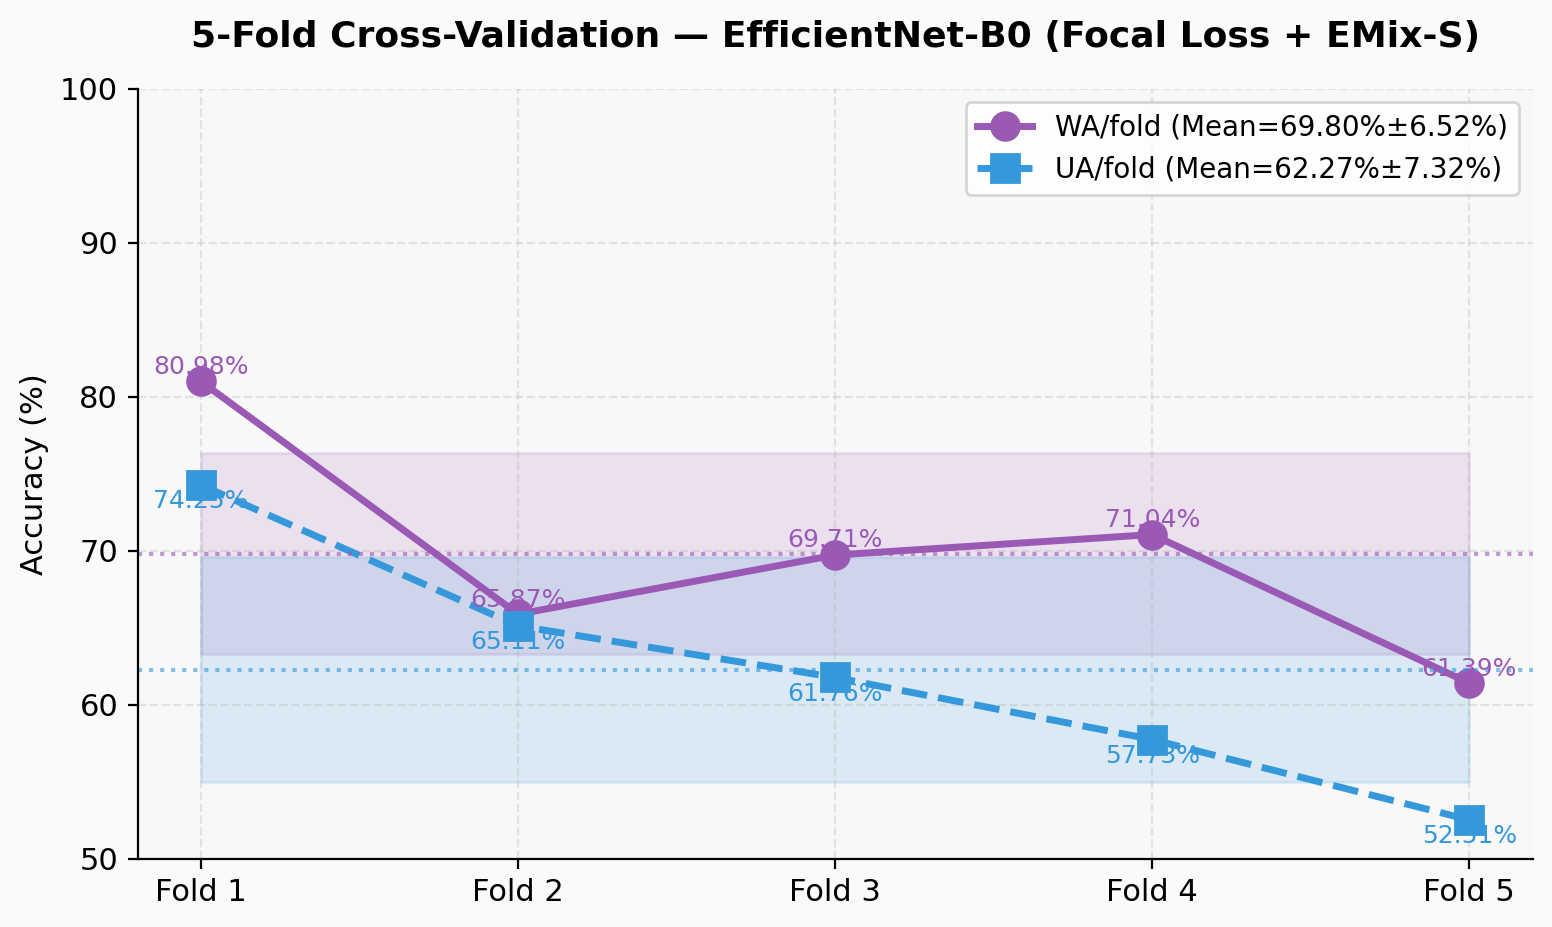
\includegraphics[width=0.8\textwidth]{crossval_results.png}
    \caption{Biểu đồ kết quả 5-Fold Cross-Validation}
    \label{fig:crossval_results}
\end{figure}

\subsection{Ví dụ chi tiết: Fold 1}

\begin{figure}[H]
    \centering
    \begin{subfigure}[b]{0.55\textwidth}
        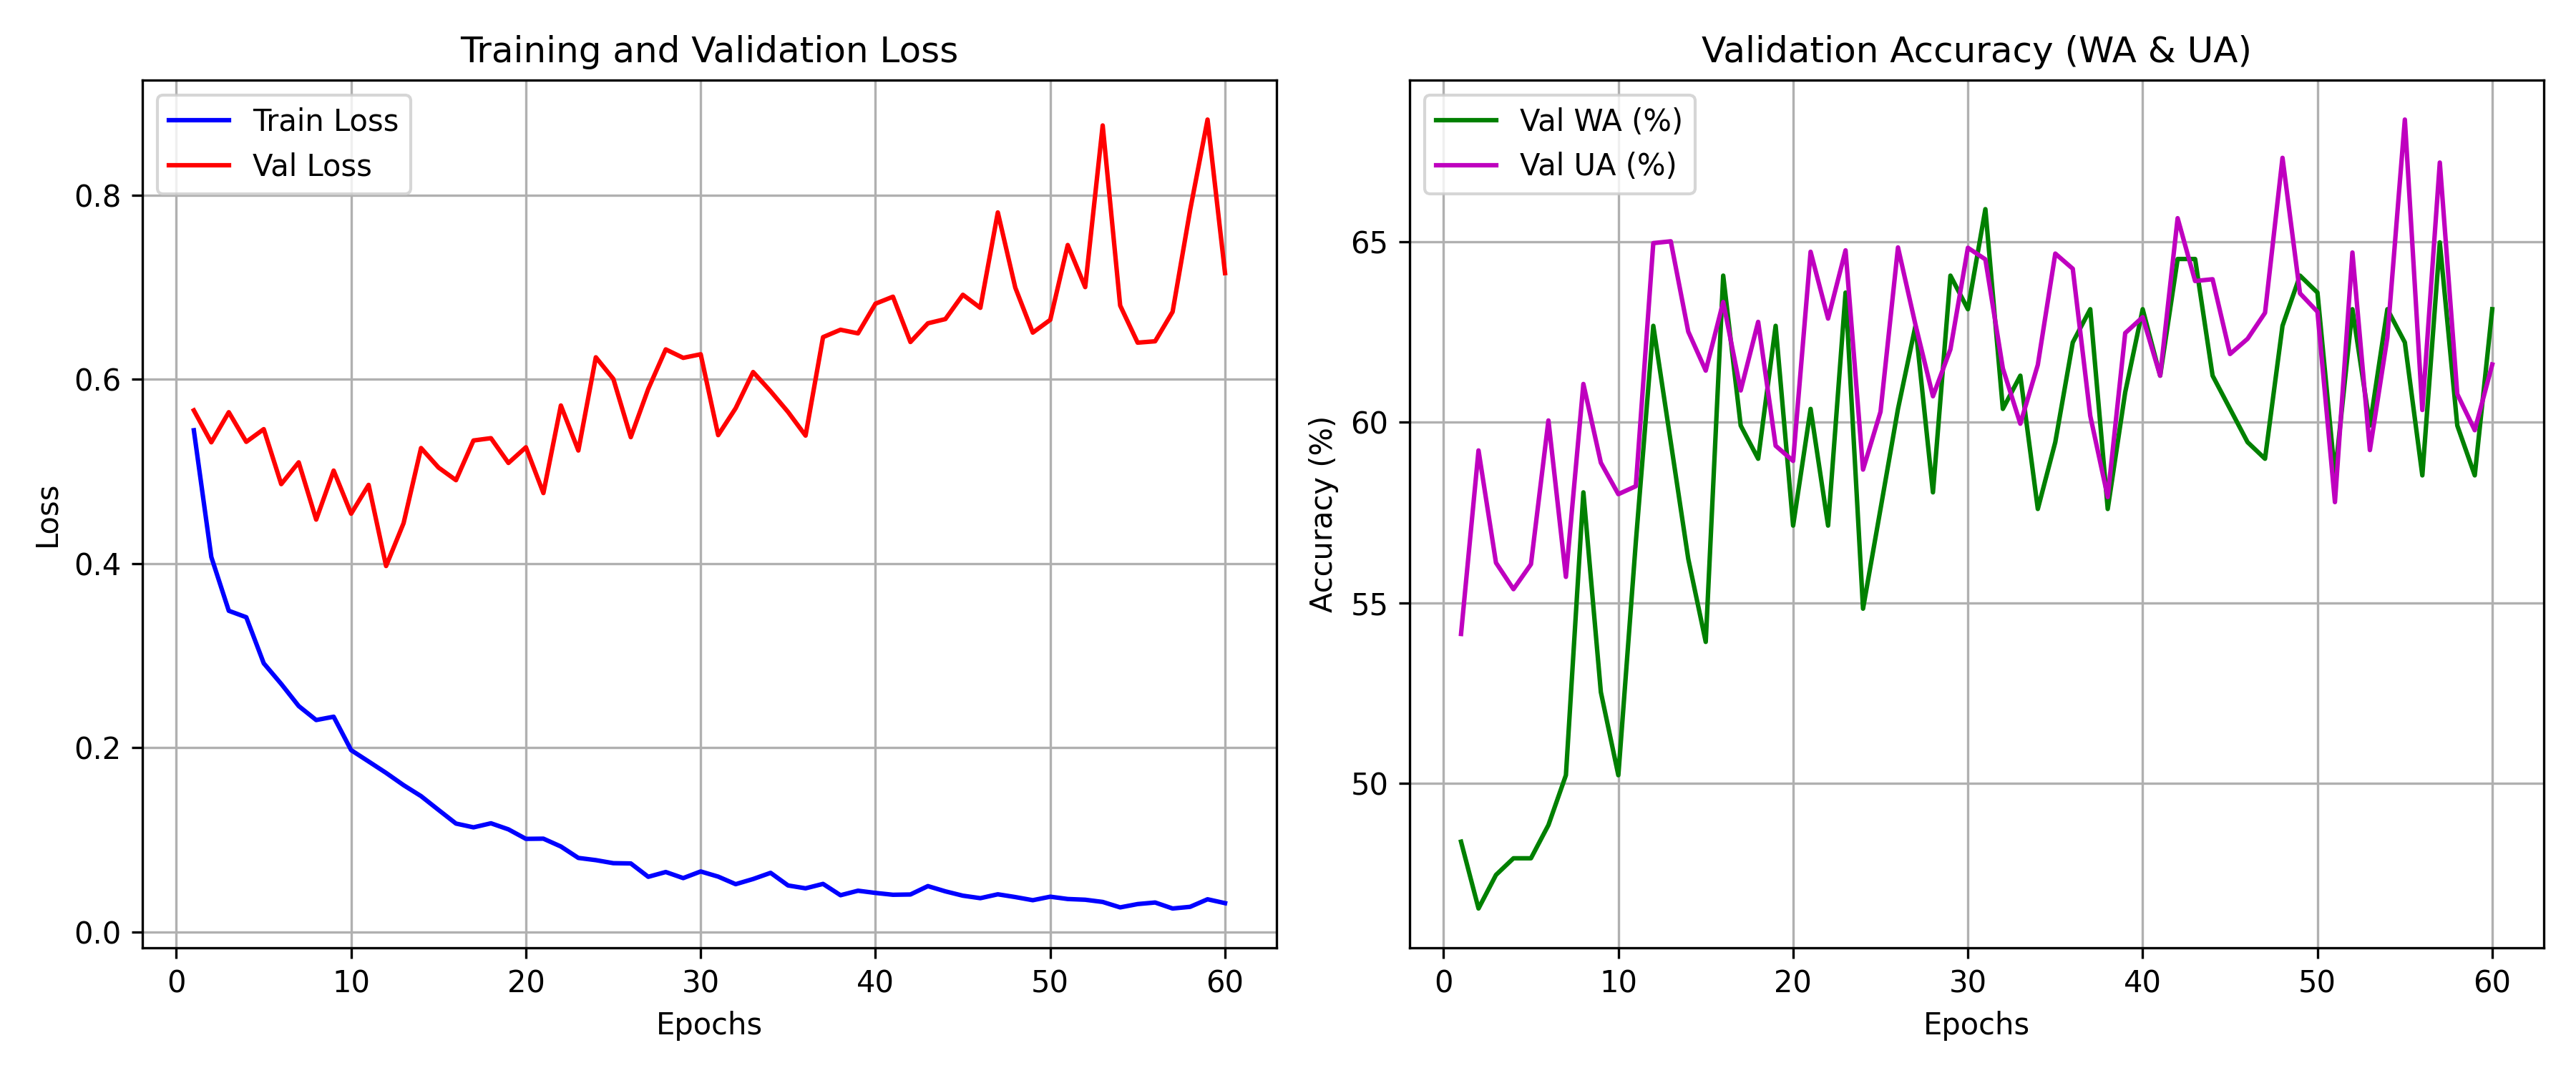
\includegraphics[width=\textwidth]{efficientnet_focal_cv_fold1_curves.png}
        \caption{Training/Validation curves}
    \end{subfigure}
    \hfill
    \begin{subfigure}[b]{0.38\textwidth}
        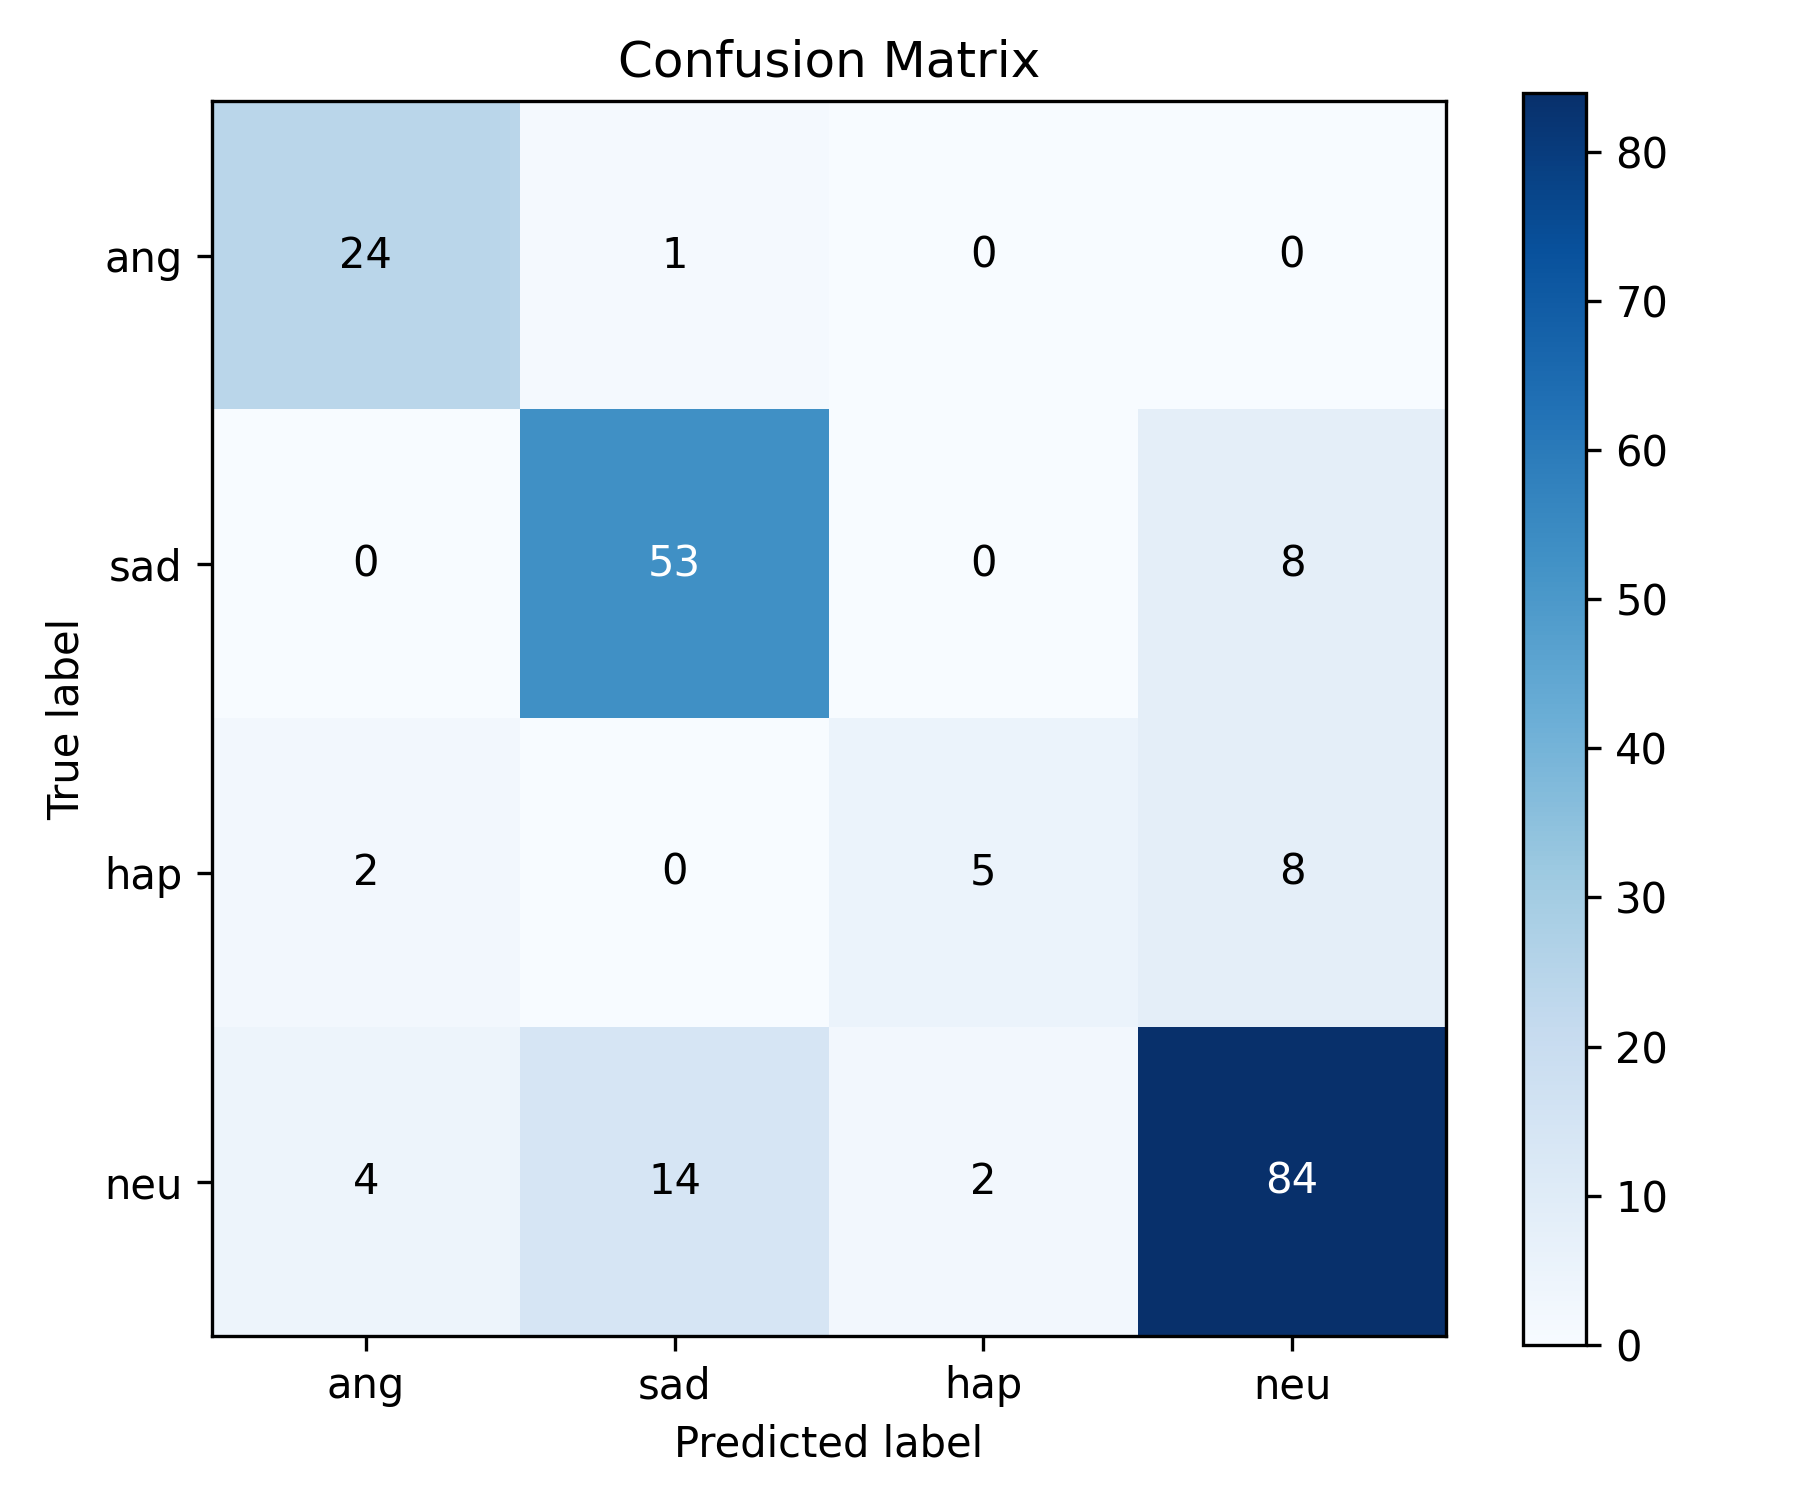
\includegraphics[width=\textwidth]{efficientnet_focal_cv_fold1_conf.png}
        \caption{Ma trận nhầm lẫn}
    \end{subfigure}
    \caption{Chi tiết Fold 1 (val=1F, test=1M): WA=80,98\%, UA=74,25\%}
    \label{fig:cv_fold1}
\end{figure}

\subsection{So sánh Single Fold vs 5-Fold}

\begin{table}[H]
\centering
\caption{So sánh phương pháp đánh giá}
\label{tab:cv_comparison}
\begin{tabular}{lccl}
\toprule
\textbf{Phương pháp} & \textbf{WA (\%)} & \textbf{UA (\%)} & \textbf{Độ tin cậy} \\
\midrule
Single Fold (val=1F, test=1M) & 80,98 & 74,25 & Thấp (phụ thuộc speaker) \\
5-Fold CV Mean $\pm$ Std & $69,80 \pm 7,29$ & $62,27 \pm 8,18$ & Cao (đại diện 10 speakers) \\
\bottomrule
\end{tabular}
\end{table}

Đồ thị biểu diễn sự biến động kết quả giữa 5 folds được minh họa tại Hình~\ref{fig:crossval_results}. Chi tiết đồ thị học tập và ma trận nhầm lẫn của thực nghiệm Fold 1 được trình bày trong Hình~\ref{fig:cv_fold1}. So sánh chi tiết hiệu năng giữa phương pháp Single Fold và 5-Fold được tổng hợp trong Bảng~\ref{tab:cv_comparison}.

Phân tích kết quả đánh giá chéo 5-Fold cho thấy chỉ số trung bình thấp hơn so với lượt đánh giá đơn lẻ khoảng 10\%, điều này phản ánh Session 1 (Fold 1) sở hữu những đặc trưng người nói dễ nhận dạng cảm xúc hơn trung bình chung của các Session còn lại. Độ lệch chuẩn mẫu khá cao của WA (7,29\%) và UA (8,18\%) phản ánh sự khác biệt lớn về giọng nói và phong cách diễn xuất giữa các speaker, vốn là đặc tính tự nhiên đầy thử thách của bài toán SER. Thực nghiệm trên Fold 5 (Test Speaker 5M) cho hiệu năng thấp nhất (WA=61,39\%, UA=52,51\%) và ghi nhận giá trị Test Loss tăng vọt lên mức 1,6825. Giá trị loss này vượt qua cả ngưỡng entropy của phép đoán ngẫu nhiên trên phân bố 4 lớp cảm xúc ($-\ln(0,25) \approx 1,386$ nats), chứng minh mô hình bị mất hiệu chuẩn (miscalibration) nghiêm trọng và đưa ra các dự đoán sai lệch với độ tự tin cực kỳ cao (overconfident misclassifications) dưới tác động của sự dịch chuyển người nói (speaker shift) ở Session 5. 

Ngoài ra, việc thiết lập tập validation luôn cố định là người nói Nữ và tập kiểm thử là người nói Nam của mỗi session là một hạn chế về tính bất đối xứng giới tính, mô hình chưa được kiểm định trên các giọng nữ độc lập gây ra sự thiên lệch trong đánh giá. Điều này cần được cải tiến bằng phân chia Leave-One-Session-Out thực thụ ở các nghiên cứu tiếp theo. Đồng thời, do độ lệch chuẩn của phép đo 5-Fold còn khá lớn ($\sim 8\%$) và chưa thực hiện các kiểm định ý nghĩa thống kê (như t-test hoặc Wilcoxon test), việc đối chiếu hiệu năng và khẳng định tính ưu việt của EfficientNet-B0 cần được diễn giải một cách thận trọng khi chuyển dịch sang các điều kiện môi trường thực tế khác.
